\documentclass[10pt,a4paper]{beamer}
\usepackage[latin1]{inputenc}
\usepackage[spanish]{babel}
\usepackage[T1]{fontenc}
\usepackage{amsmath}
\usepackage{amsfonts}
\usepackage{amssymb}
\usepackage{graphicx}
\usepackage{beamerthemesplit}
\usepackage{float}
\usepackage{multirow}
\usepackage{multicol}
\usepackage{url}
\usepackage{ragged2e}
\usepackage{array}
\usepackage{latexsym}
\usepackage{subfigure}
\usepackage{timing}
\usepackage{url}

\setbeamertemplate{footline}[frame number]
\setbeamertemplate{bibliography item}[text]
%\setbeamertemplate{subsubsection in sidebar shaded}
%{\tableofcontents[subsubsectionstyle=hide]}

%\usetheme{Montpellier}
\usetheme{Warsaw}
\decimalpoint
\renewcommand{\contentsname}{Contenido}

\begin{document}

\title{Integraci�n sem�ntica de \\ los recursos de informaci�n en \\ una memoria corporativa}
\author{Erik Alarc�n Zamora}
\date{Enero 2014. M�xico, D.F.}

\begin{frame}
\titlepage
\centering
Asesores:\\ Dra. Reyna Carolina Medina Ram�rez \\Dr. H�ctor P�rez Urbina
\\
\end{frame}
\begin{frame}
\frametitle{Contenido}
\setcounter{tocdepth}{1}  
\begin{scriptsize}\tableofcontents[]\end{scriptsize}
\end{frame}
\section{Contexto y motivaci�n}

\subsection{Memoria corporativa}
\begin{frame}
	\frametitle{Memoria Corporativa}
	%%%%%%%%%%%%%%%%%%%%%%%
	\begin{block}{Definici�n}
	\justifying 
	La representaci�n expl�cita, t�cita, consistente y persistente del conocimiento de una organizaci�n. \cite{Ontoinra2002}
	\end{block}
	
	\begin{figure}[htbp]
	\centering
	\subfigure{
	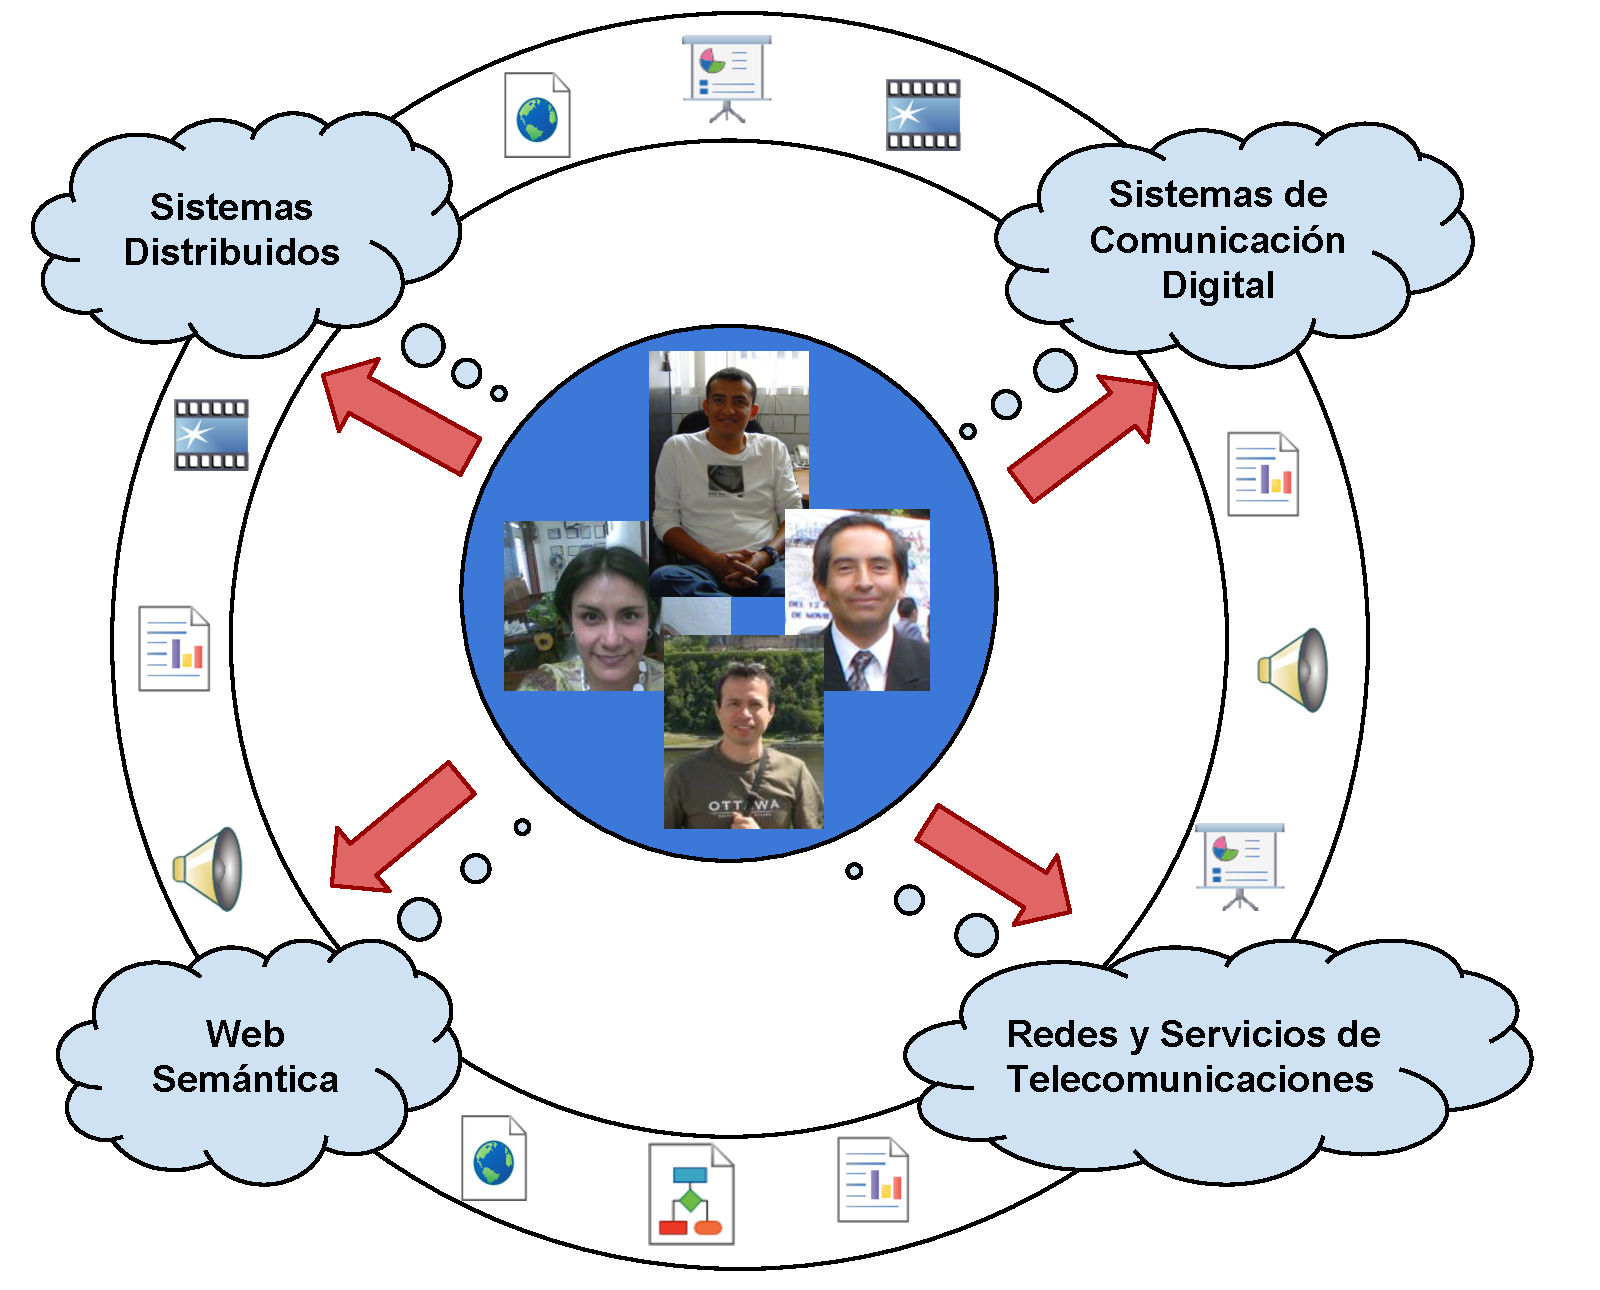
\includegraphics[scale=0.18]{ConocimientoRyT} 
	}
	\subfigure{
	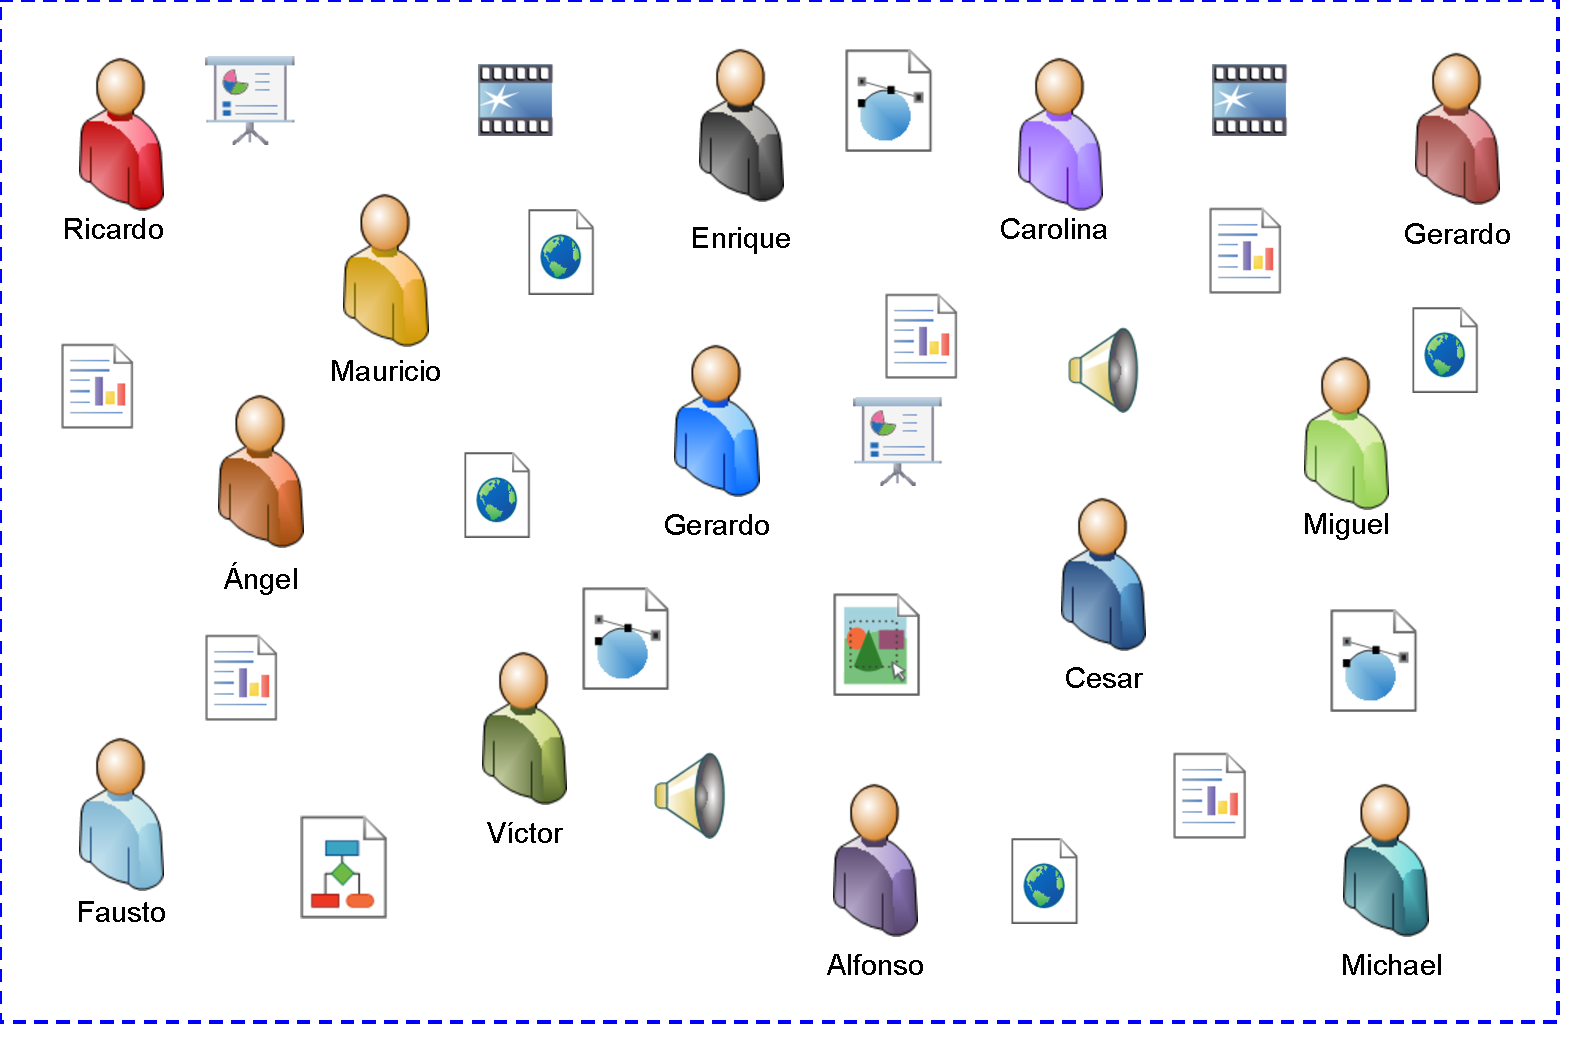
\includegraphics[scale=0.19]{EjemploMC} 
	}
	\end{figure}
	%%%%%%%%%%%%%%%%%%%%%%%
\end{frame}

\subsection{Integraci�n de la informaci�n de los recursos de informaci�n}
\begin{frame}
	\frametitle{Integraci�n de la informaci�n de los recursos de informaci�n}
	\begin{block}{Definici�n}
	\justifying
	\small La b�squeda y recuperaci�n significativa de informaci�n existente en los recursos de informaci�n para responder una consulta dada por un usuario.
	\end{block}
	
	\begin{exampleblock}{Etapas}
	\begin{enumerate}[<+-| alert@+>]
	\item \justifying \small Representar el conocimiento e informaci�n de los \textit{recursos de informaci�n}.
	\item \justifying \small Buscar y recuperar informaci�n, mediante la interrogaci�n de la representaci�n de conocimiento (modelo).
	\end{enumerate}
	\end{exampleblock}
	
	\begin{figure}
	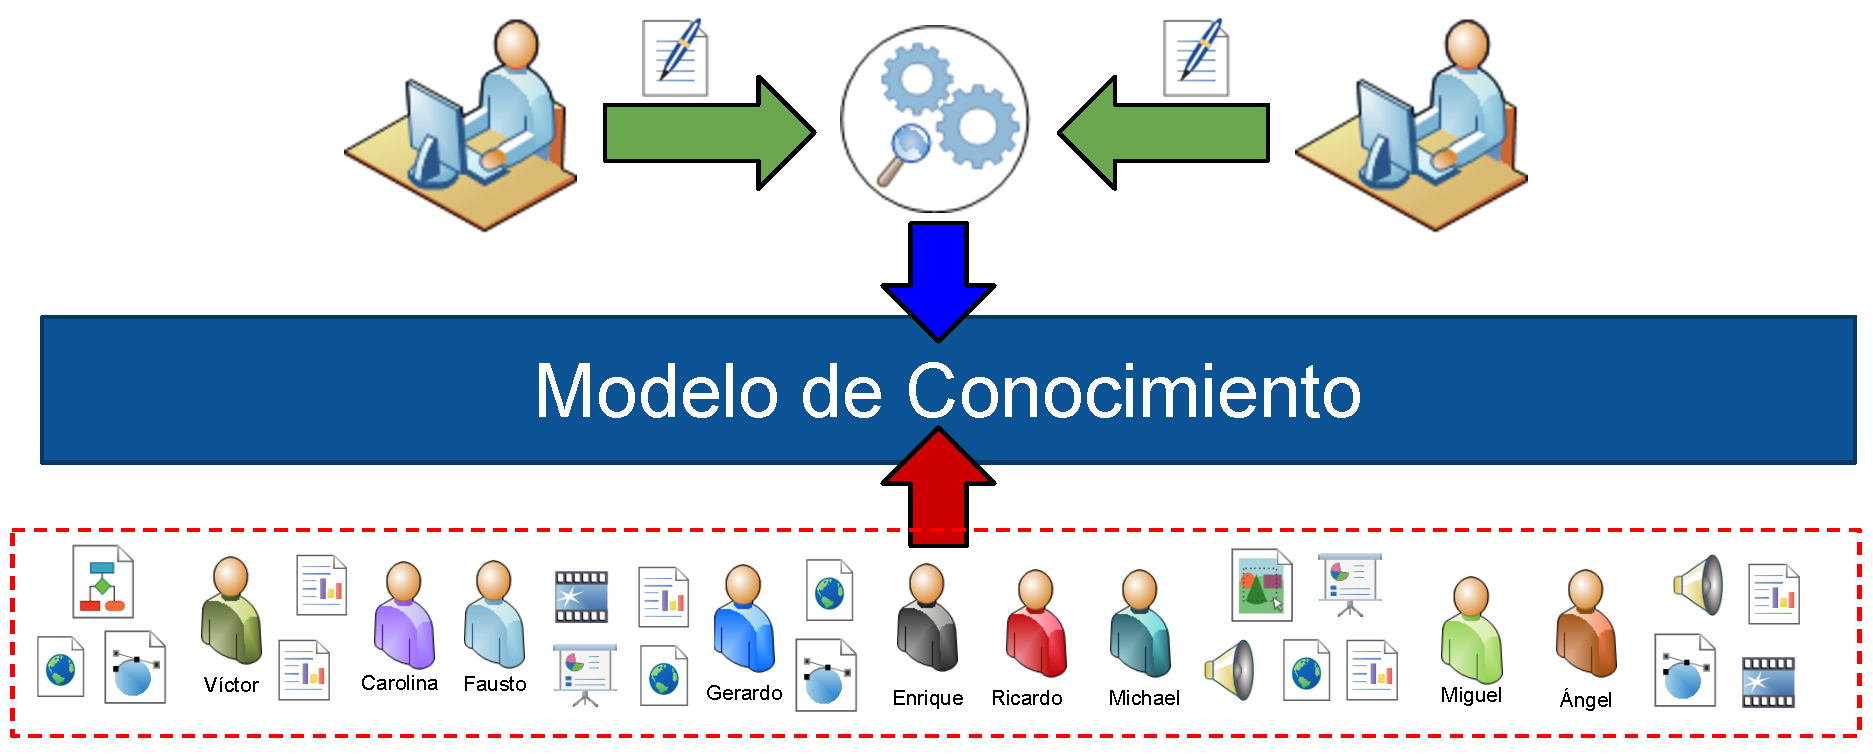
\includegraphics[scale=0.24]{IntegracionSemantica} 
	\end{figure}
\end{frame}

\subsection{Tecnolog�as Sem�nticas}
\begin{frame}
	\frametitle{Tecnolog�as Sem�nticas}
	\begin{block}{Definici�n}
	\justifying 
	\textit{Un conjunto de metodolog�as, lenguajes, aplicaciones, herramientas y est�ndares para suministrar u obtener el significado de las palabras, informaci�n y las relaciones entre �stos}. \begin{scriptsize}\cite{SemTecRetr}\end{scriptsize}
	\end{block}
	
	\begin{figure}
	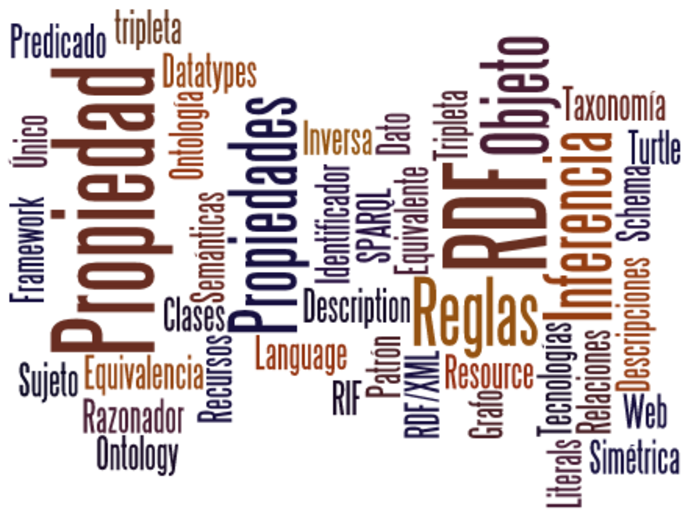
\includegraphics[scale=0.42]{TSWords} 
	\end{figure}
\end{frame}

\subsection{Integraci�n sem�ntica de recursos de informaci�n}
\begin{frame}
	\frametitle{Integraci�n sem�ntica de recursos de informaci�n}
	\begin{figure}
	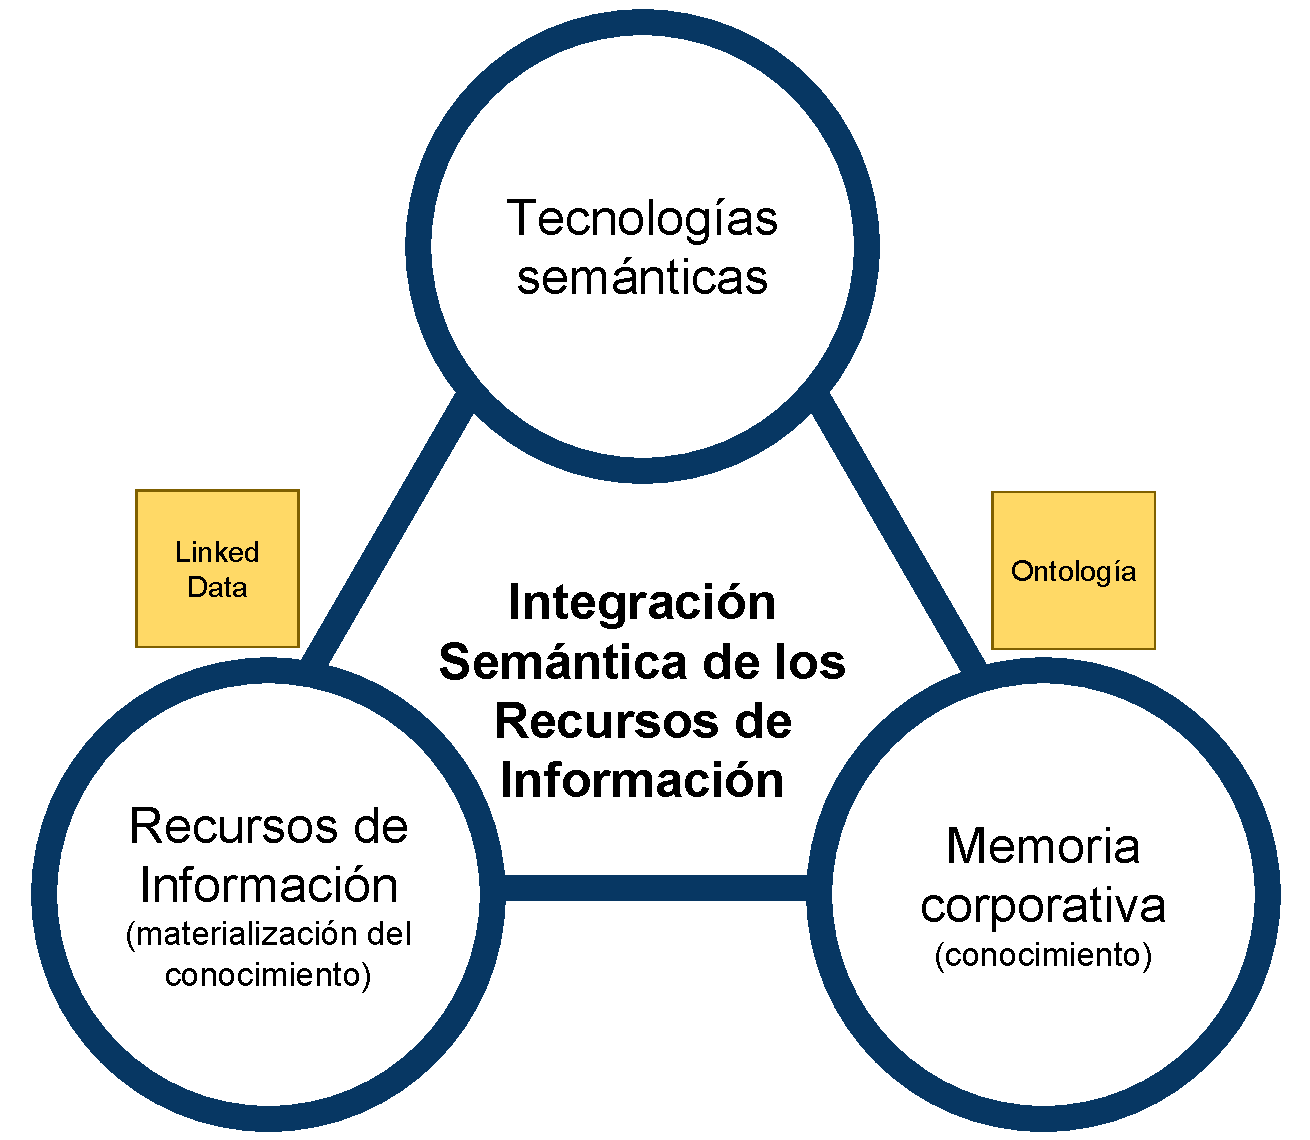
\includegraphics[scale=0.38]{ISRIMC} 
	\end{figure}
\end{frame}

\subsection{Estado del Arte}
\begin{frame}
	\frametitle{Estado del Arte}
	\begin{block}{Ejes claves}
	\begin{enumerate}
	\item \justifying Integraci�n de la informaci�n a partir del uso de tecnolog�as sem�nticas.
	\item \justifying B�squeda, recuperaci�n y publicaci�n de la informaci�n desde una ontolog�a.
	\item \justifying Gesti�n de una memoria corporativa.
	\end{enumerate}
	\end{block}
	
	\begin{figure}
	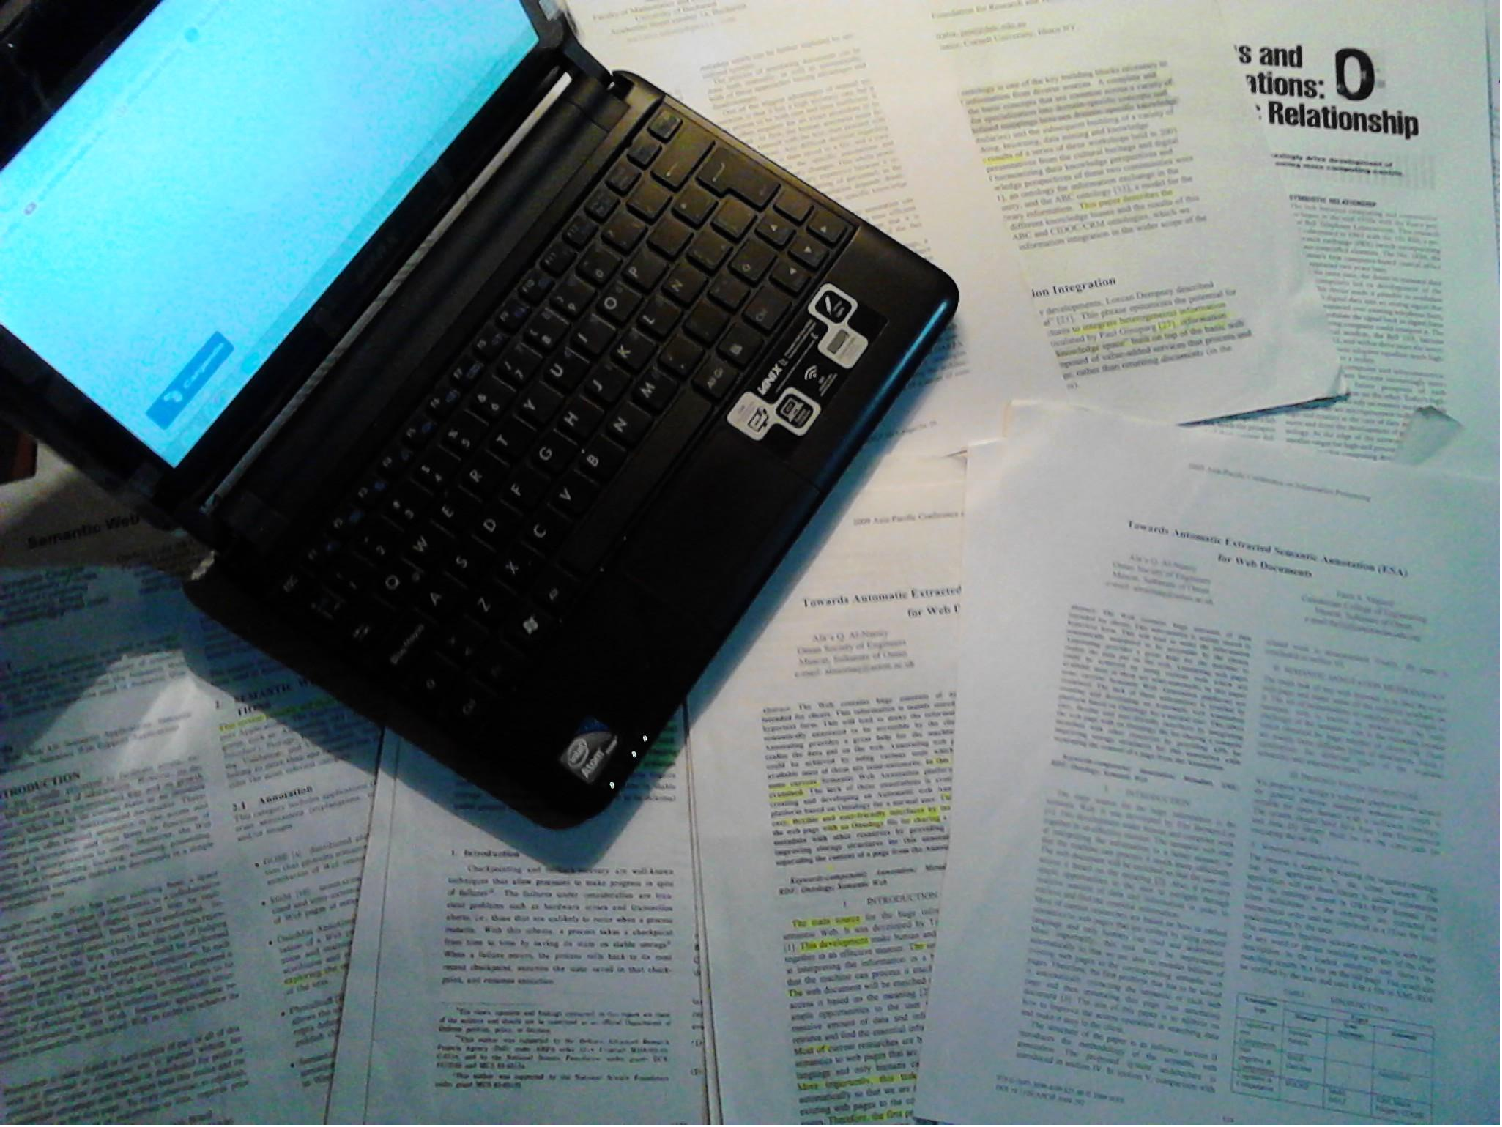
\includegraphics[scale=0.15]{EstadoArte} 
	\end{figure}
\end{frame}

\begin{frame}
	\frametitle{Comparativa}
	\begin{figure}
	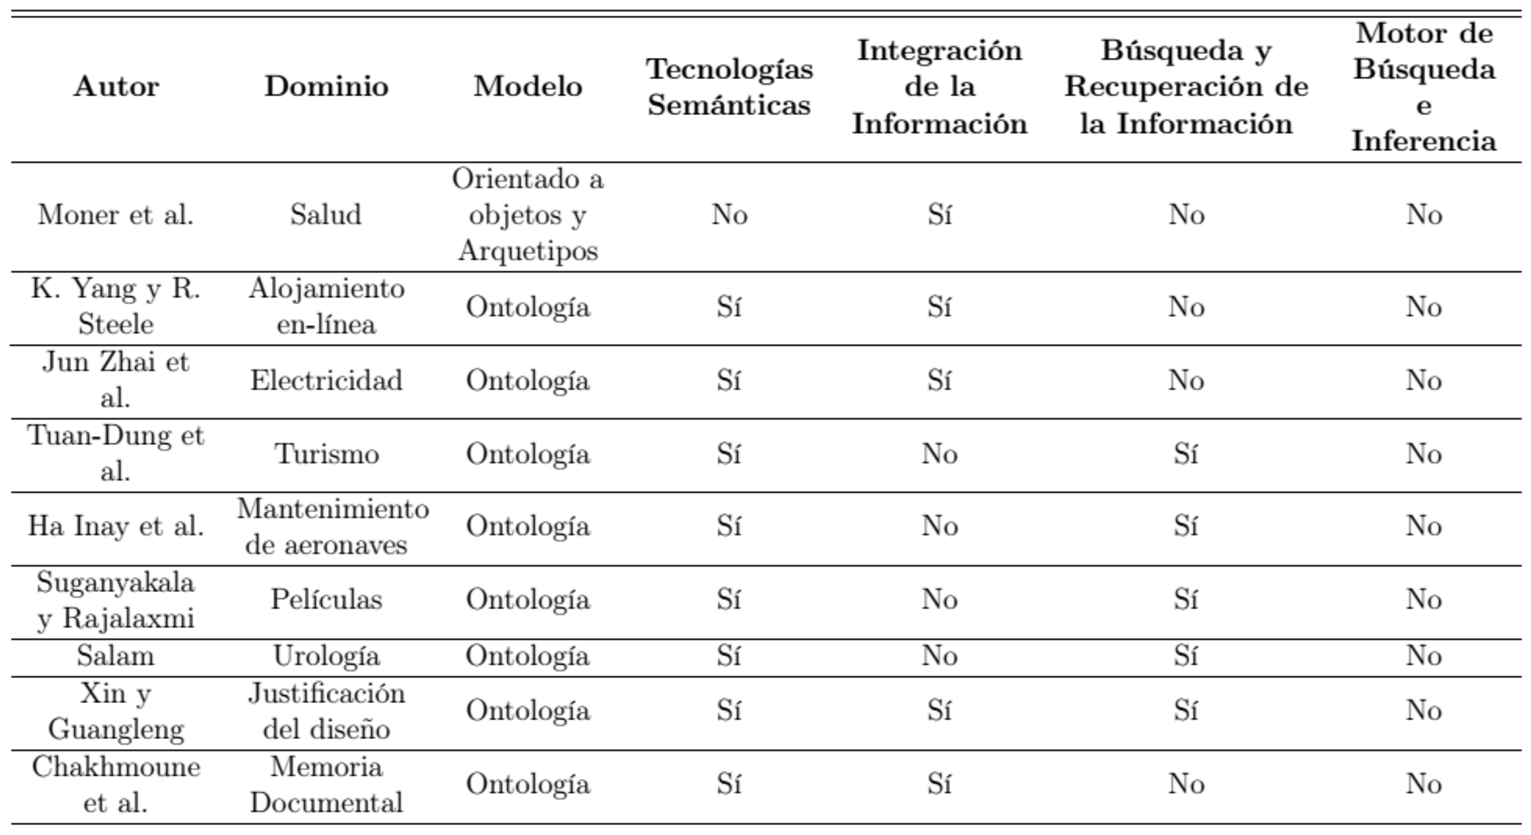
\includegraphics[scale=0.42]{TablaEOA} 
	\end{figure}
\end{frame}
\section{Descripci�n del Problema}

\subsection{Pregunta Investigaci�n}
\begin{frame}
	\frametitle{Pregunta Investigaci�n} 
	\begin{exampleblock}{}
	\justifying 
	\textit{�Las \textbf{tecnolog�as sem�nticas} son viables para solucionar la \textbf{integraci�n sem�ntica} de los \textbf{recursos de informaci�n} de una \textbf{memoria corporativa}?}
	\end{exampleblock}
	
	\begin{figure}
	
\includegraphics[scale=0.4]{PreguntaInv} 
	\end{figure}
\end{frame}

\subsection{Objetivos}
\begin{frame}
	\frametitle{Objetivos} 
	\begin{alertblock}{Objetivo Principal}
	\justifying 
	Contribuir a la \textit{integraci�n sem�ntica} de los \textit{recursos de informaci�n} en \textit{una memoria corporativa}, mediante el uso de las \textit{tecnolog�as sem�nticas}.
	\end{alertblock}
	
	\begin{block}{Objetivos Particulares}
	\begin{enumerate}
	\item \justifying \small Un \textbf{\textit{marco de referencia}} para la \textit{integraci�n sem�ntica} de los \textit{recursos de informaci�n}.
	\item \justifying \small Un \textbf{\textit{modelo sem�ntico}} que representa el \textit{conocimiento expl�cito e impl�cito} de los \textit{recursos de informaci�n}.
	\item \justifying \small Un \textbf{\textit{prototipo de interfaz gr�fica de usuario}} que permita a los usuarios consultar y visualizar la informaci�n de los recursos de informaci�n, interrogando un modelo sem�ntico.
	\item \justifying \small La evaluaci�n de la calidad de los \textbf{\textit{resultados recuperados}} y los \textbf{\textit{tiempos de procesamiento}} de la \textit{integraci�n sem�ntica}.
	\end{enumerate}
	\end{block}
\end{frame}

\subsection{Metodolog�a}
\begin{frame}
	\frametitle{Metodolog�a I}
	\begin{block}{Marco de Referencia}
	\begin{enumerate}
	\item \justifying \small Identificar los \textit{casos de uso}.
	\item \justifying \small Evaluar las \textit{herramientas sem�nticas}.
	\item \justifying \small Conformar los \textit{recurso de informaci�n} de la \textit{memoria corporativa}.
	\end{enumerate}
	
	\begin{exampleblock}{Modelo Sem�ntico}
	\begin{enumerate}
	\setcounter{enumi}{3}
	\item \justifying \small Representar el \textit{conocimiento expl�cito} de los \textit{recursos de informaci�n} en un \textit{modelo sem�ntico} (ontolog�a).
	\item \justifying \small Enriquecer el \textit{modelo sem�ntico} con \textit{reglas de inferencia}.
	\end{enumerate}
	\end{exampleblock}
	
	\begin{enumerate}
	\setcounter{enumi}{5}
	\item \justifying \small Escribir las principales \textit{consultas} en la sintaxis correspondiente.
	\item \justifying \small Emplear un razonador para hacer expl�cito el conocimiento impl�cito.
	\item \justifying \small Buscar y recuperar informaci�n en la memoria corporativa, interrogando el modelo sem�ntico inferido.
	\end{enumerate}
	\end{block}
\end{frame}

\begin{frame}
	\frametitle{Metodolog�a II}	
	\begin{block}{Prototipo de interfaz gr�fica de usuario}	
	\begin{enumerate}
	\setcounter{enumi}{8}
	\item \justifying \small Construir el \textit{prototipo de interfaz de usuario} para la (b�squeda y navegaci�n) de los usuarios en un modelo sem�ntico.
	\end{enumerate}
	\end{block}
	
	\begin{block}{Evaluaci�n}
	\begin{enumerate}
	\setcounter{enumi}{9}
	\item \justifying \small Evaluar la calidad de los resultados con y sin inferencia.
	\item \justifying \small Evaluar los \textit{tiempos promedios} de consulta sobre modelos con/sin inferencia.
	\end{enumerate}
	\end{block}
\end{frame}

\subsection{Hip�tesis}
\begin{frame}
	\frametitle{Hip�tesis}
	\begin{block}{}
	\justifying 
	\textbf{El uso de las \textit{tecnolog�as sem�nticas} es adecuado para lograr la \textit{integraci�n sem�ntica} de \textit{recursos de informaci�n} en una \textit{memoria corporativa}}.
	\end{block}
	
	\begin{figure}
	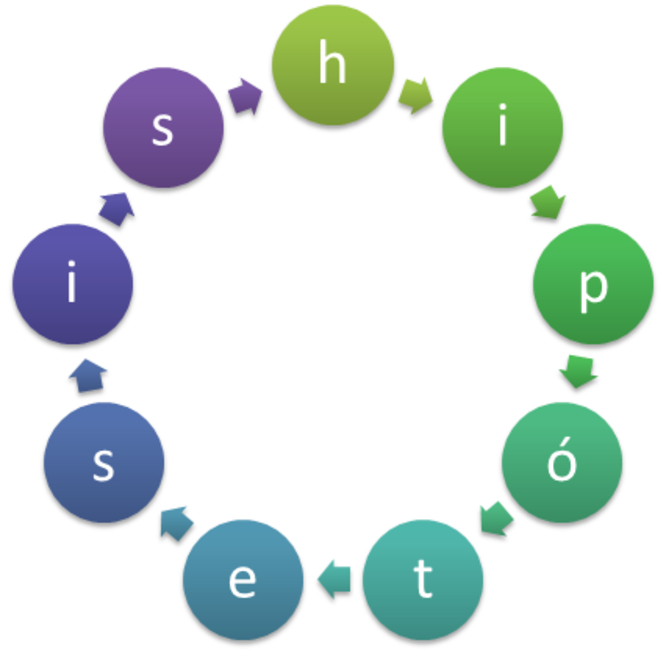
\includegraphics[scale=0.45]{hipotesis} 
	\end{figure}
\end{frame}

\subsection{Aportaciones}
\begin{frame}
	\frametitle{Aportaciones}
	\begin{enumerate}
	\item \justifying Un \textit{marco de referencia} para lograr la \textit{integraci�n sem�ntica} de \textit{recursos de informaci�n}.
    \item \justifying Un modelo sem�ntico que representa el conocimiento de una memoria corporativa.
    \item \justifying  Un prototipo (interfaz gr�fica de usuario) para la interacci�n amigable (b�squeda y consulta de informaci�n) de los usuarios con el modelo sem�ntico.
    \item \justifying Los resultados de nuestra evaluaci�n experimental.
    \item \justifying Un par de scripts para la generaci�n autom�tica y controlada de descripciones (conocimiento expl�cito) de los \textit{recursos de informaci�n}.
	\end{enumerate}
\end{frame}
%%%%%%%%%%%%%%%%%%%%%%%%%%%%%%%%%%%%%%%%%%%%%%%%%%%%%%%%%%%%%%%%%%%%%%%%%%%%%%
\section{Integraci�n Sem�ntica de una Memoria Corporativa}
%%%%%%%%%%%%%%%%%%%%%%%%%%%%%%%%%%%%%%%%%%%%%%%%%%%%%%%%%%%%%%%%%%%%%%%%%%%%%%
\begin{frame}
	\frametitle{Marco de Referencia}
	\begin{block}{Etapas}
		\begin{enumerate}
		\item \justifying Representar las caracter�sticas y/o relaciones de los \textit{recursos de informaci�n} mediante el est�ndar RDF, para construir un modelo sem�ntico.
		\item \justifying Introducir \textit{reglas de inferencia} en el modelo sem�ntico, para enriquecer con \textit{conocimiento impl�cito} de los \textit{recursos de informaci�n} y del dominio de la memoria.
		\item \justifying Buscar y recuperar informaci�n en el modelo sem�ntico para responder un conjunto consultas SPARQL.
		\end{enumerate}
	\end{block}
\end{frame}
%%%%%%%%%%%%%%%%%%%%%%%%%%%%%%%%%%%%%%%%%%%%%%%%%%%%%%%%%%%%%%%%%%%%%%%%%%%%%%

%%%%%%%%%%%%%%%%%%%%%%%%%%%%%%%%%%%%%%%%%%%%%%%%%%%%%%%%%%%%%%%%%%%%%%%%%%%%%%
\begin{frame}
	\frametitle{Arquitectura de la Integraci�n Sem�ntica}	
	\begin{figure}
	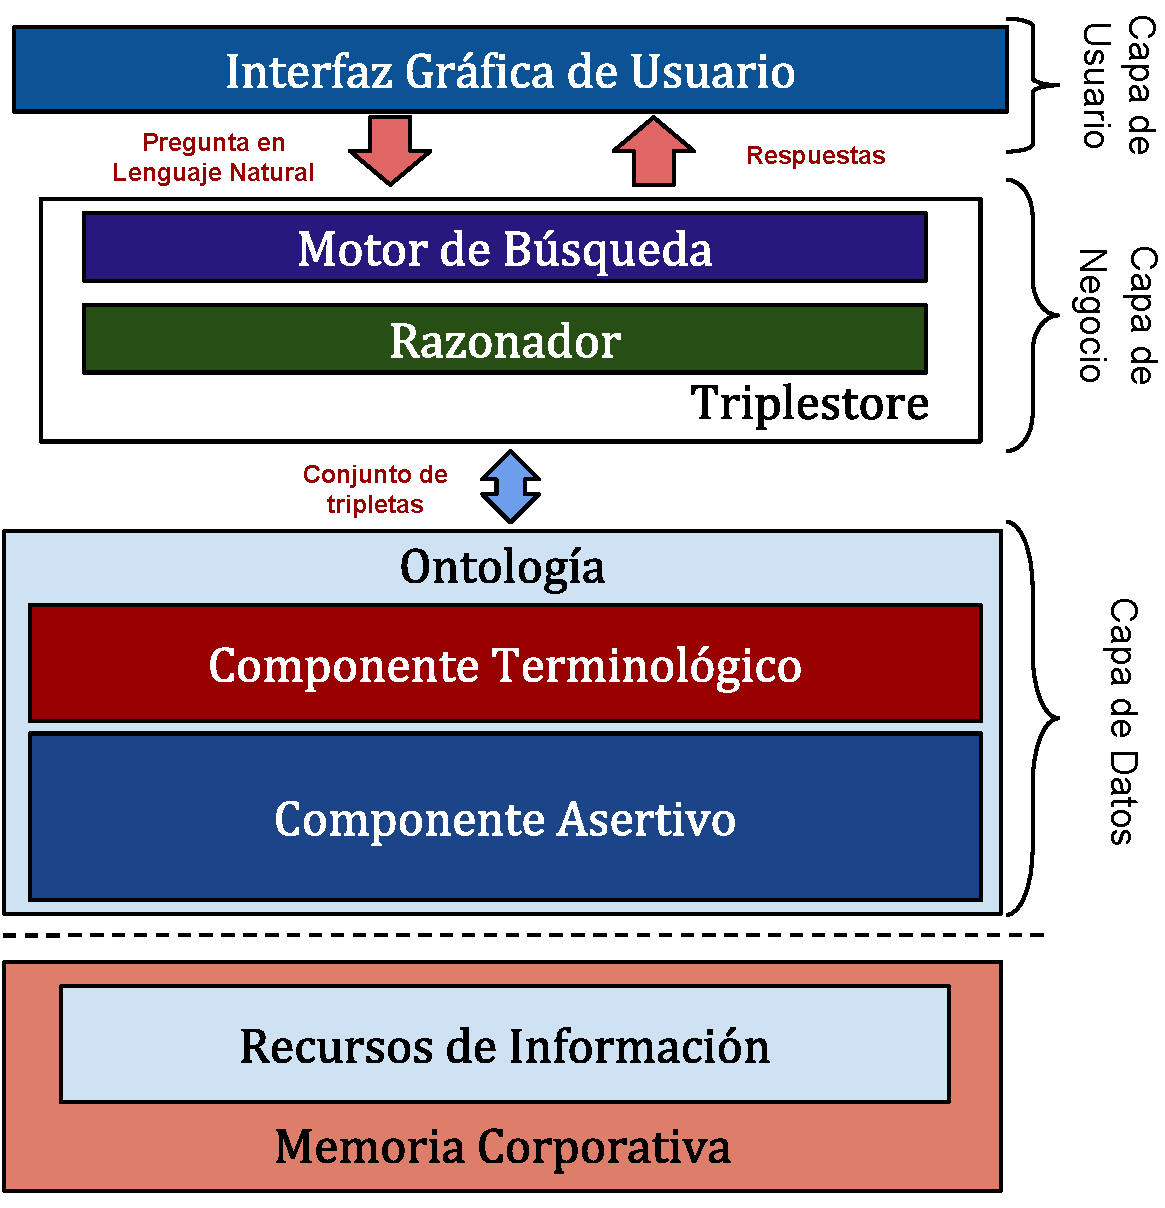
\includegraphics[scale=0.33]{Arquitectura} 
	\end{figure}
\end{frame}
%%%%%%%%%%%%%%%%%%%%%%%%%%%%%%%%%%%%%%%%%%%%%%%%%%%%%%%%%%%%%%%%%%%%%%%%%%%%%%

%%%%%%%%%%%%%%%%%%%%%%%%%%%%%%%%%%%%%%%%%%%%%%%%%%%%%%%%%%%%%%%%%%%%%%%%%%%%%%
\begin{frame}
	\frametitle{Casos de Uso}
	
	\begin{block}{}
		\begin{itemize}
		\item \justifying \textbf{\textit{Cartograf�a de Competencias}} es la b�squeda y recuperaci�n de informaci�n significativa de las personas a partir de las caracter�sticas personales y profesionales de las mismas.
		\item \justifying \textbf{\textit{B�squeda de Recursos Digitales}} es la b�squeda y recuperaci�n de informaci�n significativa de los documentos y archivos multimedia a partir del contenido de los mismos.
		\end{itemize}
	\end{block}
	
	\begin{figure}
	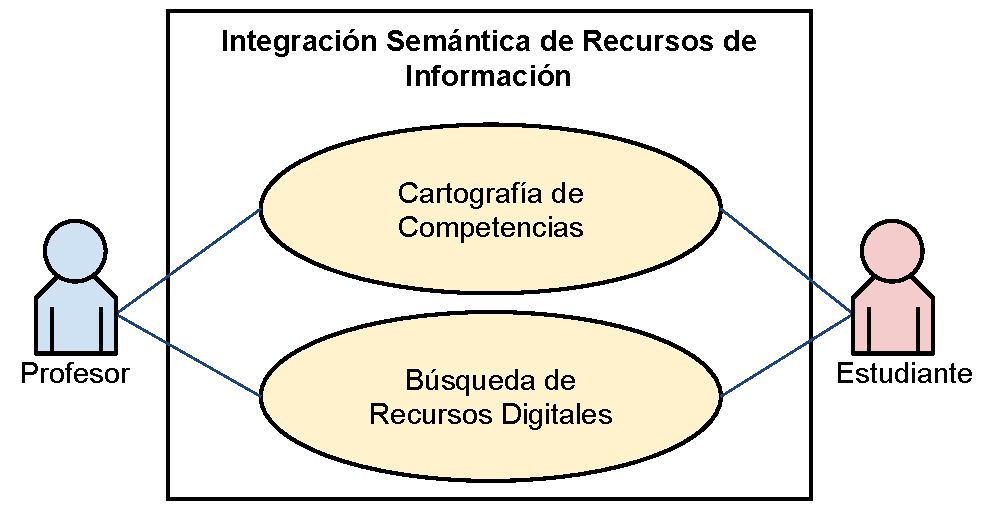
\includegraphics[scale=0.56]{CasosUso} 
	\end{figure}
\end{frame}
%%%%%%%%%%%%%%%%%%%%%%%%%%%%%%%%%%%%%%%%%%%%%%%%%%%%%%%%%%%%%%%%%%%%%%%%%%%%%%

%%%%%%%%%%%%%%%%%%%%%%%%%%%%%%%%%%%%%%%%%%%%%%%%%%%%%%%%%%%%%%%%%%%%%%%%%%%%%%
\subsection{Representaci�n el Conocimiento}
\subsubsection{Identificar los principales recursos de informaci�n}
\begin{frame}
	\frametitle{Identificar los principales recursos de informaci�n}	
	\begin{figure}
	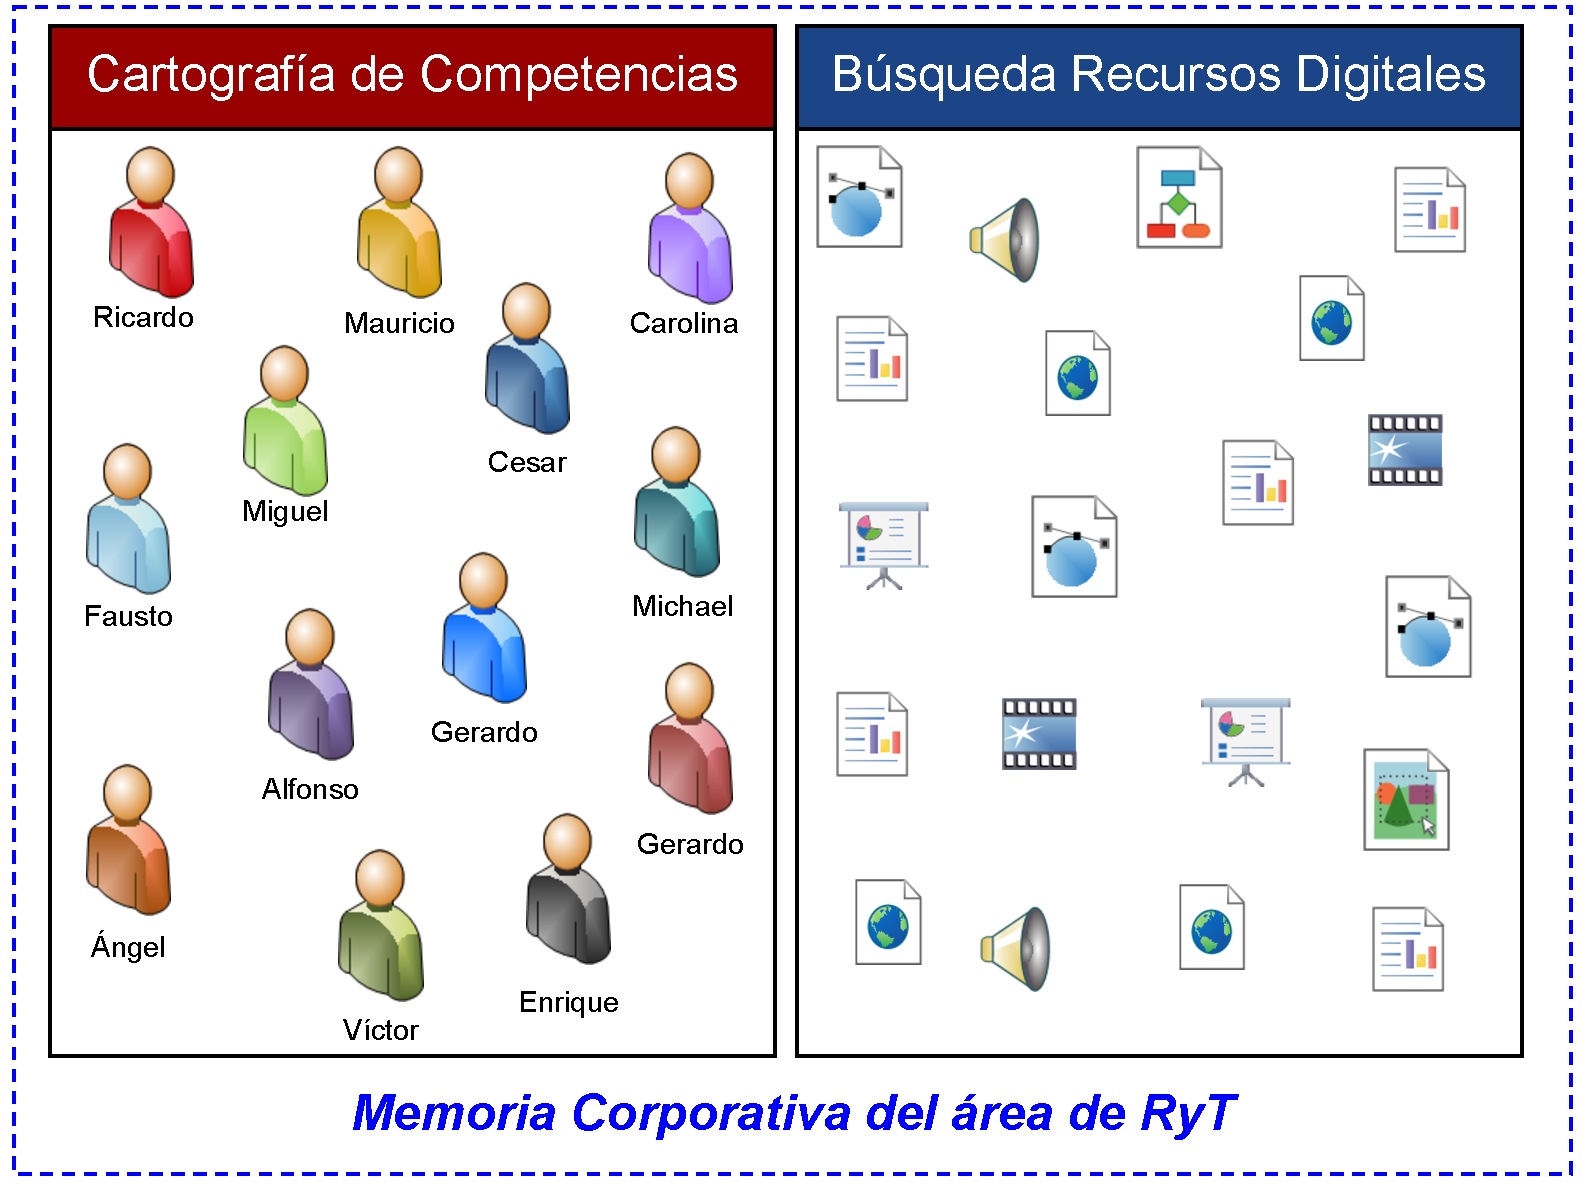
\includegraphics[scale=0.33]{CasosUsoMC} 
	\end{figure}
\end{frame}

\subsubsection{Adquirir y expresar el conocimiento de los recursos de informaci�n}
\begin{frame}
	\frametitle{Adquirir y expresar el conocimiento de los recursos de informaci�n}	
	\begin{figure}
	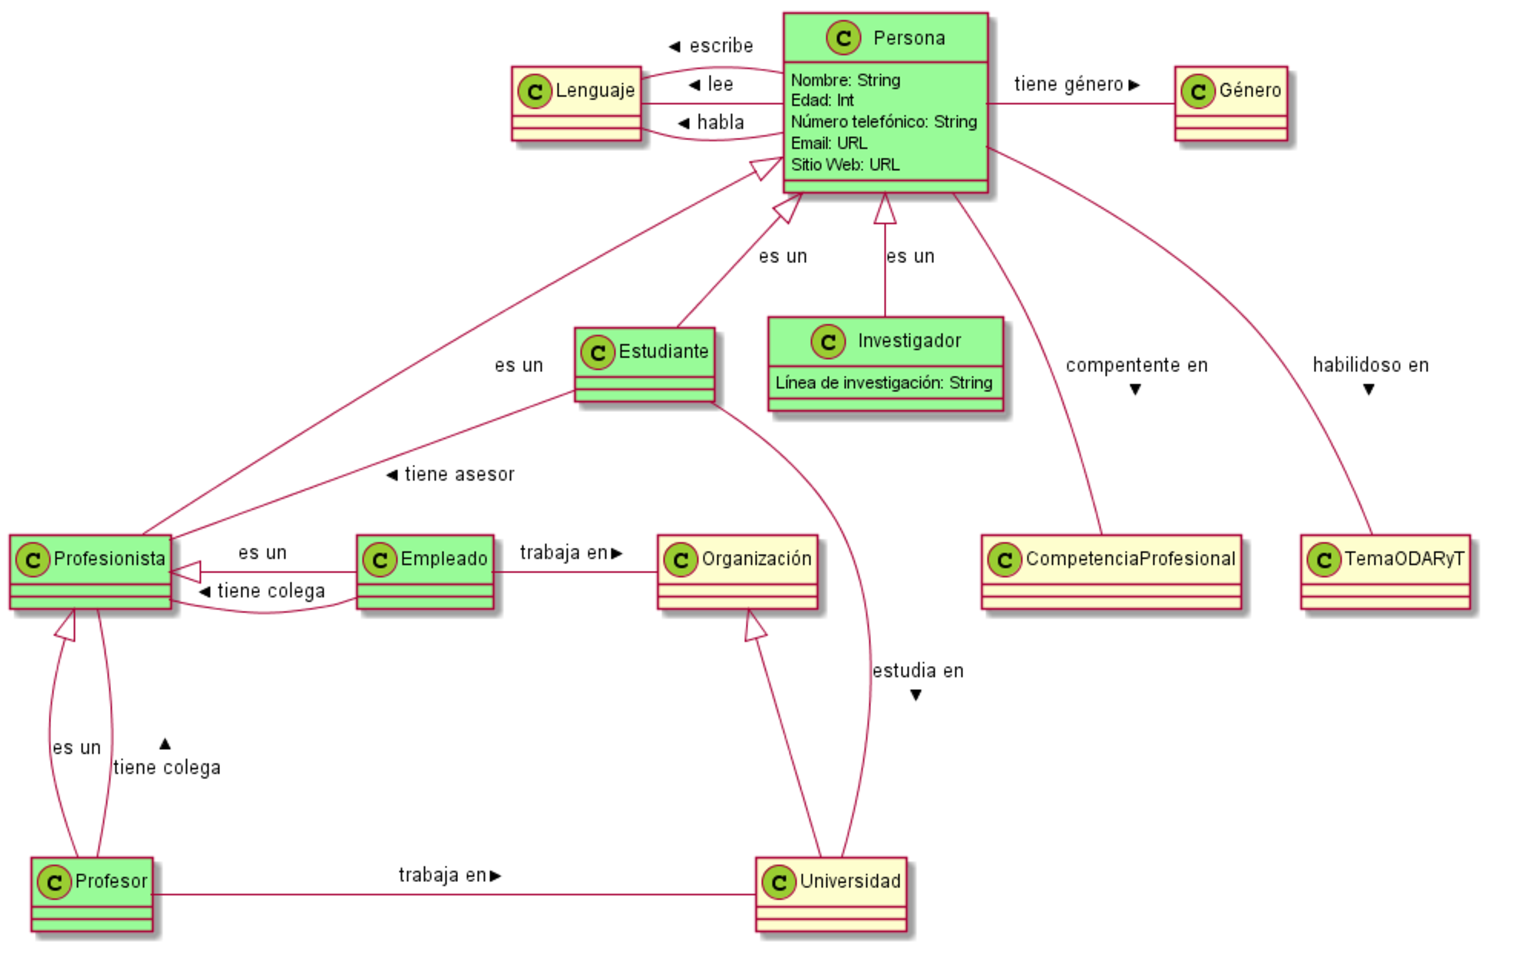
\includegraphics[scale=0.38]{CasoUsoCartComp} 
	\end{figure}
\end{frame}

\subsubsection{Representar el conocimiento e informaci�n mediante el est�ndar RDF}
\begin{frame}
	\frametitle{Representar el conocimiento e informaci�n mediante el est�ndar RDF}
	
	\begin{block}{Definici�n}
	\justifying 
	Marco gen�rico para describir el conocimiento e informaci�n expl�cita de los recursos mediante sus caracter�sticas y relaciones. \begin{scriptsize}\cite{SurvSemWeb2012}\end{scriptsize}
	\end{block}
	
	\begin{block}{Actividades en la representaci�n del conocimiento}
	\begin{enumerate}
	\item \justifying Asignar un \textit{identificador �nico de recursos} (URI) a cada \textit{recurso de informaci�n} en la \textit{memoria corporativa}.
	\item \justifying Asignar un URI a cada caracter�stica y/o relaci�n (propiedad) de de los \textit{recursos de informaci�n}.
	\item \justifying Generar las tripletas RDF asociadas a las descripciones de los recursos de informaci�n.
	\end{enumerate}
	\end{block}
%	\begin{figure}
%	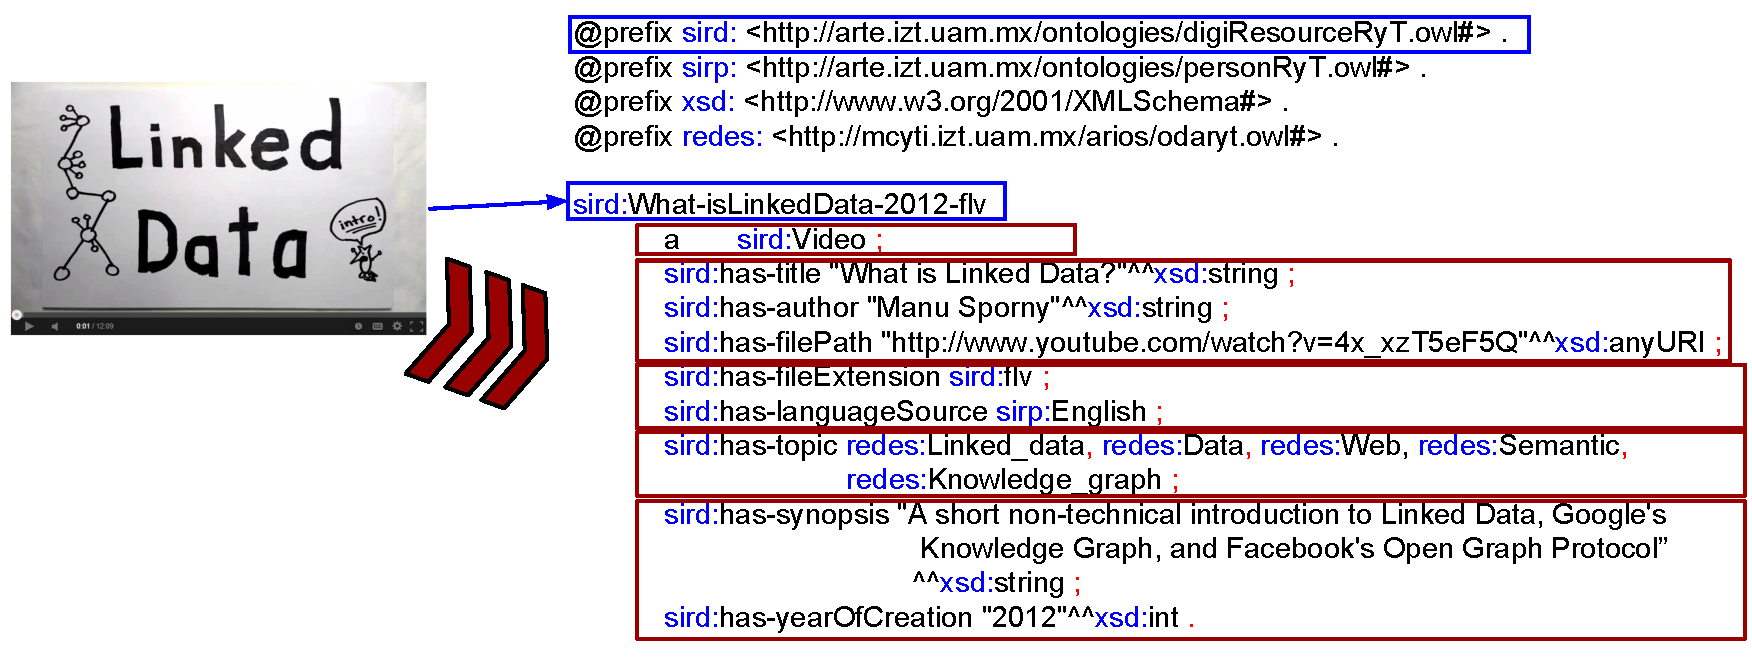
\includegraphics[scale=0.38]{Vid2RDF}
%	\end{figure}
	%%%%%%%%%%%%%%%%%%%%%%%
\end{frame}

\begin{frame}
	\frametitle{Representar el conocimiento e informaci�n mediante el est�ndar RDF}
	\begin{figure}
	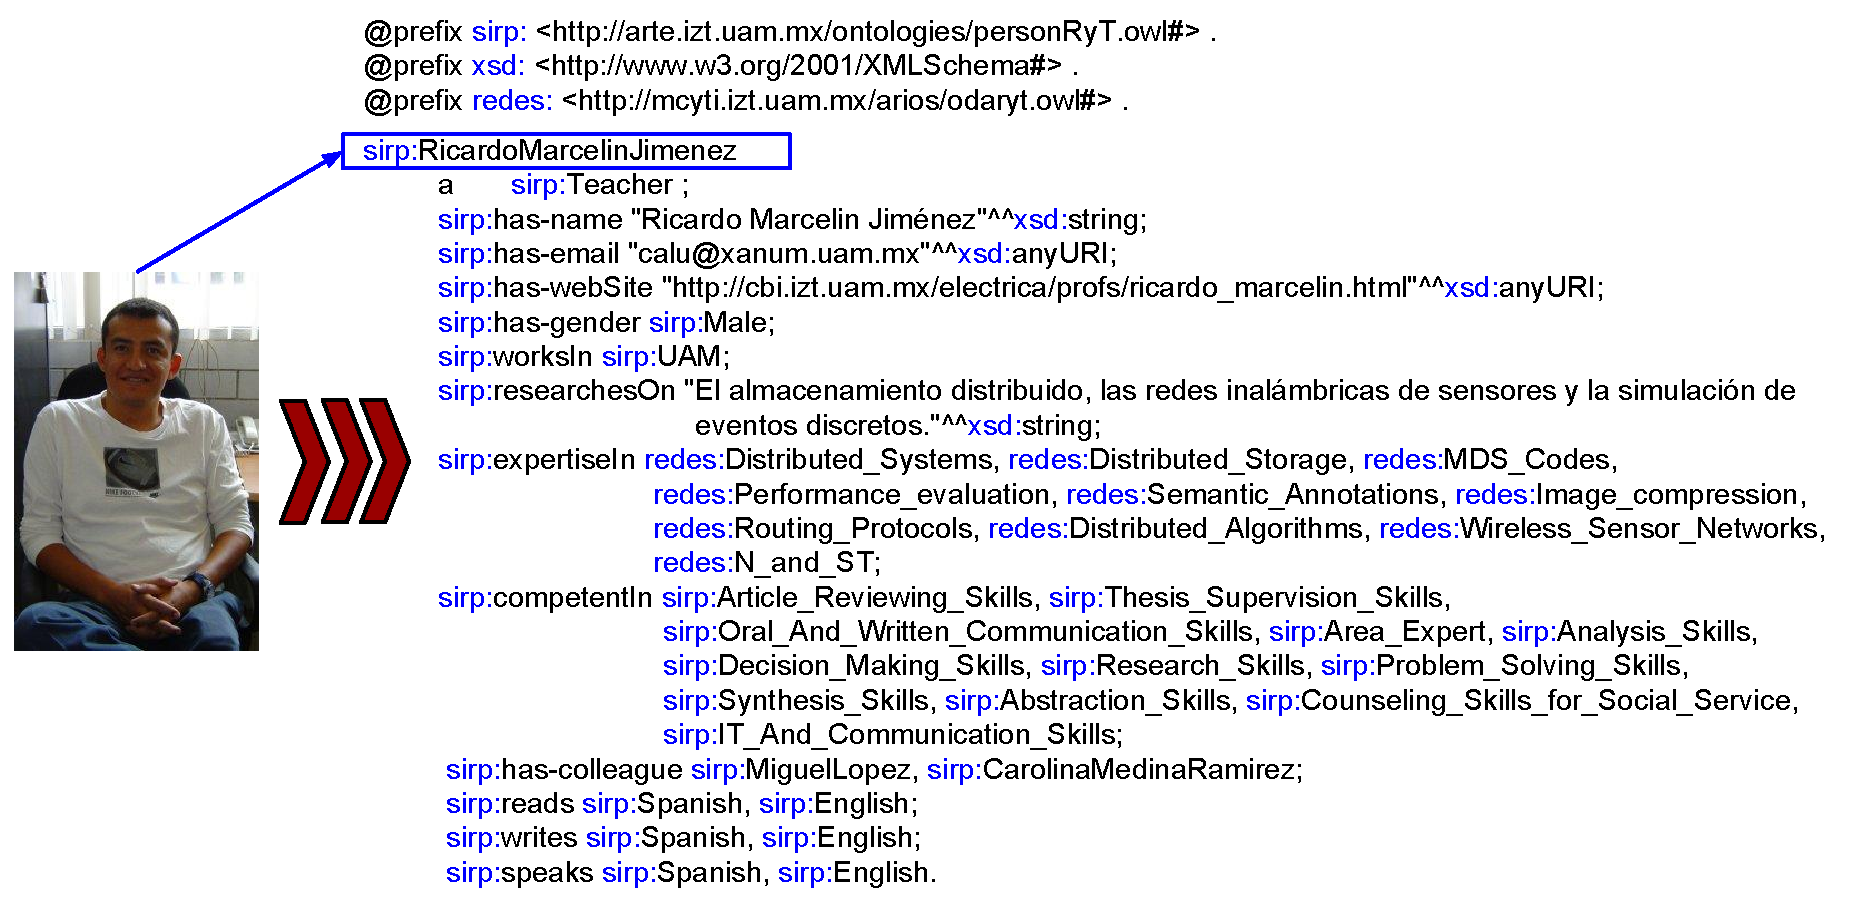
\includegraphics[scale=0.35]{Person2RDF}
	\end{figure}
\end{frame} 

\begin{frame}
	\frametitle{Representar el conocimiento e informaci�n mediante el est�ndar RDF}
	\begin{figure}
	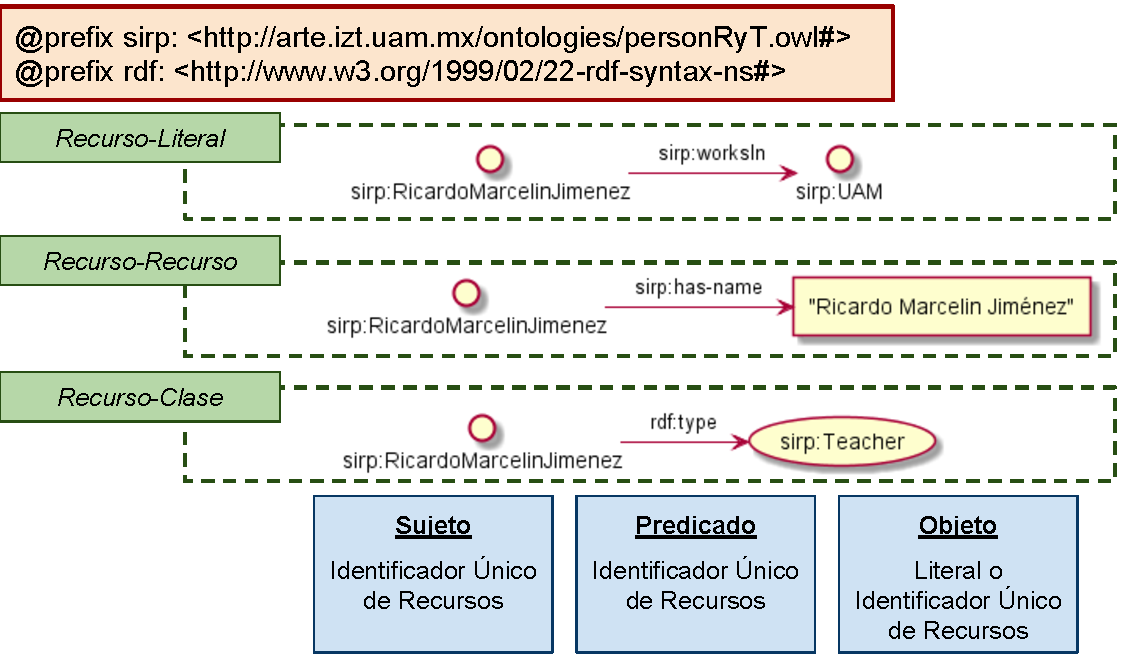
\includegraphics[scale=0.45]{Tripletas} 
	\end{figure}
\end{frame}

\begin{frame}
	\frametitle{Representar el conocimiento e informaci�n mediante el est�ndar RDF}
	\begin{figure}
	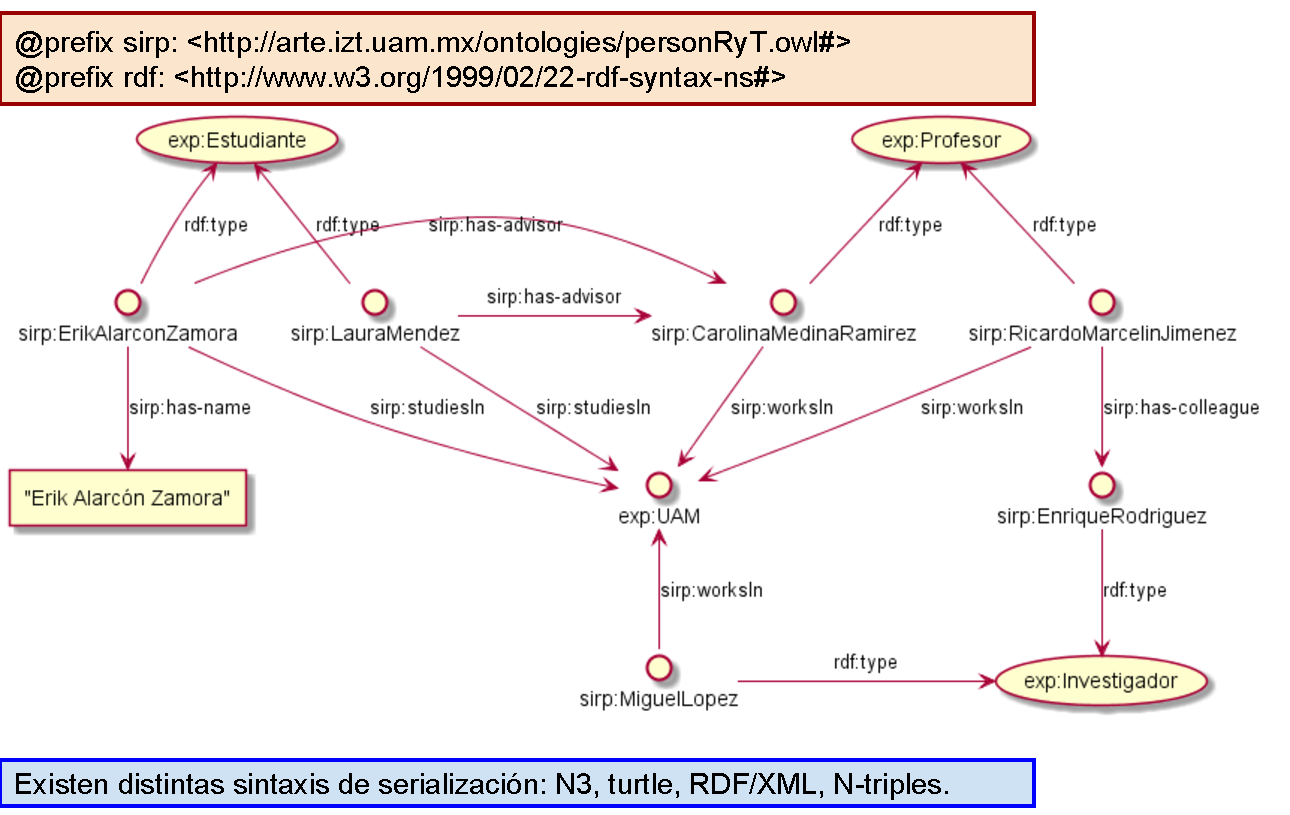
\includegraphics[scale=0.48]{GrafoRDF} 
	\end{figure}
\end{frame}

%%%%%%%%%%%%%%%%%%%%%%%%%%%%%%%%%%%%%%%%%%%%%%%%%%%%%%%%%%%%%%%%%%%%%%%%%%%%%%

\subsection{Enriquecer el conocimiento en el modelo sem�ntico}
\begin{frame}
	\frametitle{Ontolog�a}
	%%%%%%%%%%%%%%%%%%%%%%%%%%%%
	\begin{alertblock}{Definici�n}
	\justifying 
	Una definici�n formal, expl�cita y compartida de los conceptos, as� como las relaciones de un determinado dominio. \begin{scriptsize}\cite{Gruber}\end{scriptsize}
	\end{alertblock}
	
	\begin{block}{Componentes}
	\begin{itemize}
	\item \justifying \textbf{\textit{Componente Asertivo (ABox)}} est� constituido por descripciones que afirman que los individuos son instancias de una clase o propiedad.
	\item \justifying \textbf{\textit{Componente Terminol�gico (TBox)}} describe las clases y propiedades relevantes, as� como las reglas de inferencia que permiten aprovechar la manera en que las instancias se relacionan entre s�.
	\end{itemize}
	\end{block}
	%%%%%%%%%%%%%%%%%%%%%%%%%%%%
\end{frame}

\begin{frame}
	\frametitle{Axiomatizaci�n}	
	\begin{block}{Reglas de inferencia o Axiomas}
	\justifying 
	Expresiones para enriquecer un grafo RDF con conocimiento impl�cito.\\
	\end{block}
	
	\begin{block}{Lenguajes}
	Especificaciones para describir clases, propiedades e individuos.
	\begin{itemize}
	\item \justifying \textit{RDF Schema \textbf{RDF(S)}}
	\item \justifying \textit{Web Ontology Language \textbf{OWL}} 
	\end{itemize}
	\end{block}
	
	\begin{figure}
	
\includegraphics[scale=0.4]{PrefijosRDFSOWL}
	\end{figure}
	
	\begin{block}
	\justifying
	\textit{Lo que es obvio para un humano, no lo es para una maquina}.
	\end{block}
\end{frame}

%\begin{frame}
%	\frametitle{Enriquecer el conocimiento en el modelo sem�ntico}
%	\begin{block}{}
%	\justifying
%	Para cada \textit{caso de uso} debe encontrarse el respectivo conjunto de axiomas (TBox).
%	\end{block}
%	
%	\begin{figure}
%	
\includegraphics[scale=0.4]{PrefijosRDFSOWL}
%	\end{figure}
%\end{frame}
	
\subsubsection{Herencia de Clases}
\begin{frame}[allowframebreaks]
	\frametitle{Herencia de Clases}
	\begin{block}{Subclase (rdfs:subClassOf)}
	\justifying
	Afirma que una \textit{clase A} se subsume por una \textit{clase B}, es decir, la clase A es un caso particular de la \textit{clase B}. En este caso, las instancias de la clase A son instancias de la clase B.
	\end{block}
	
	\begin{figure}
	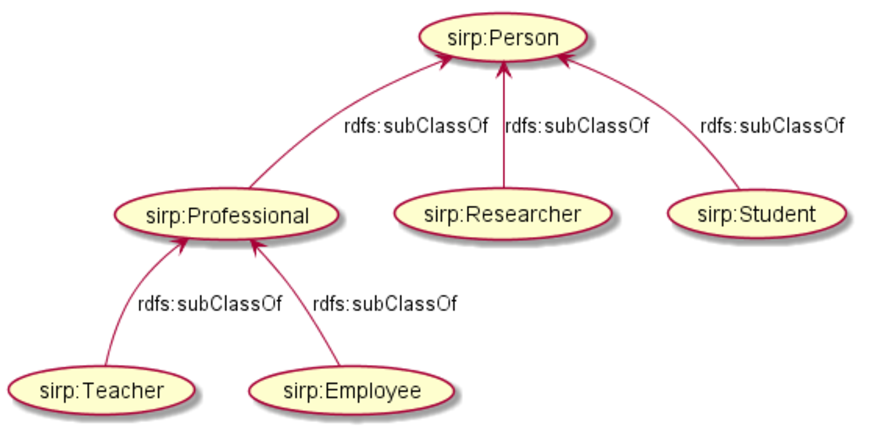
\includegraphics[scale=0.5]{HerenClassCartComp}
	\end{figure}
	%%%%%%%%%%%%%%%%%%%%%%%
	
	\begin{figure}
	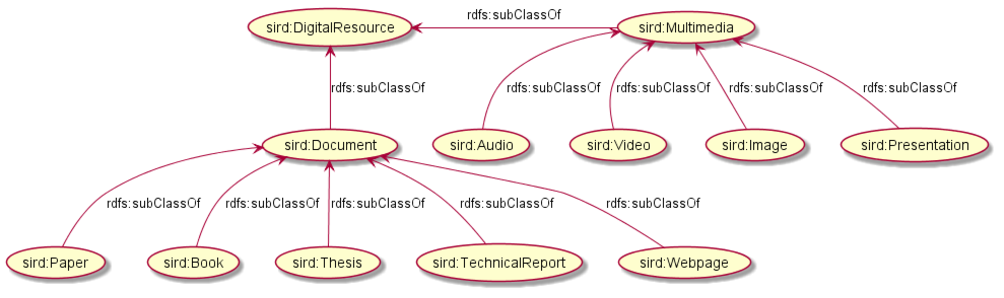
\includegraphics[scale=0.68]{HerenClassRecDigi}
	\end{figure}
	%%%%%%%%%%%%%%%%%%%%%%%
	
	\begin{figure}
	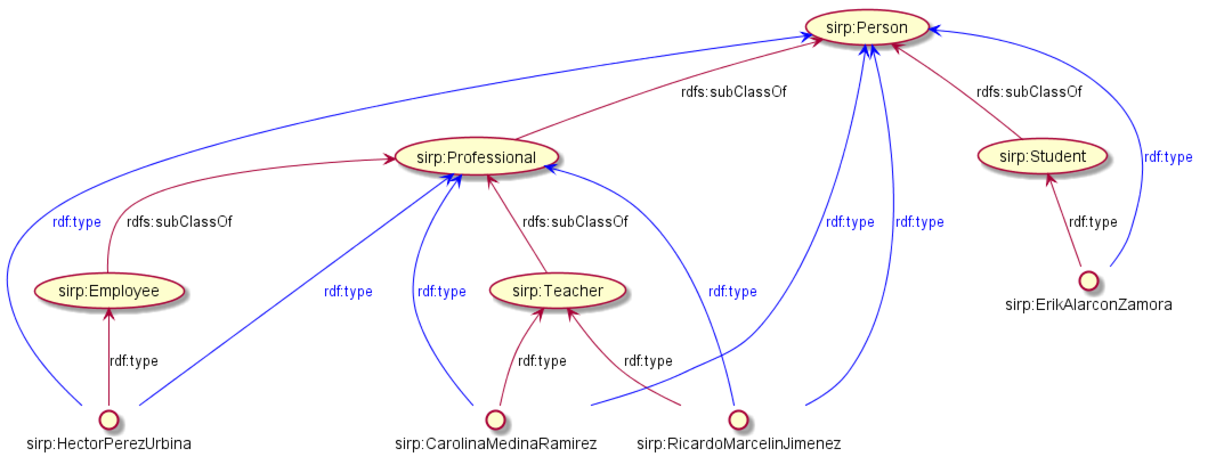
\includegraphics[scale=0.57]{EjmpInfSubClass}
	\end{figure}
	%%%%%%%%%%%%%%%%%%%%%%%
\end{frame}

\subsubsection{Herencia de Propiedades}
\begin{frame}[allowframebreaks]
	\frametitle{Herencia de Propiedades}
	\begin{block}{Subpropiedad (rdfs:subPropertyOf)}
	\justifying
	Afirma que todos los recursos que se relacionan por la \textit{propiedad X}, tambi�n se relacionan por la \textit{propiedad Y}.
	\end{block}
	
	\begin{figure}
	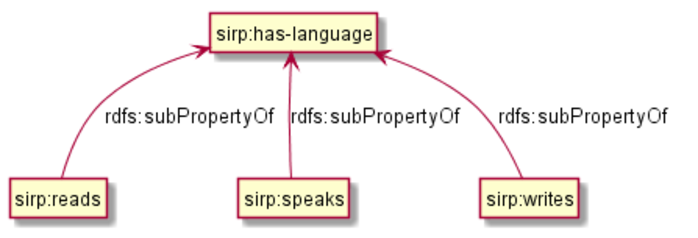
\includegraphics[scale=0.57]{HerPropLang}
	\end{figure}
		
	\begin{figure}
	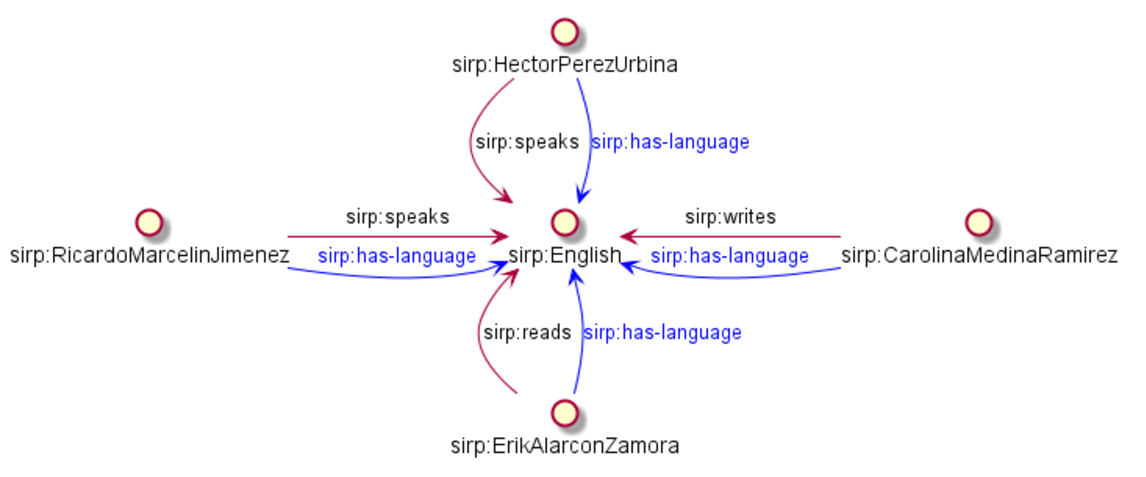
\includegraphics[scale=0.55]{EjmpInfProp}
	\end{figure}
	%%%%%%%%%%%%%%%%%%%%%%%
\end{frame}

\subsubsection{Dominio y Rango en las Propiedades}
\begin{frame}[allowframebreaks]
	\frametitle{Dominio y Rango en las Propiedades}
	\begin{block}{Dominio (rdfs:domain)}
	\justifying
	Especifica qu� clase se aplica a una propiedad.
	\end{block}
	
	\begin{block}{Rango (rdfs:range)}
	\justifying
	Especifica los valores (clase o tipo de literal) que puede asumir una propiedad.
	\end{block}
	
	\begin{figure}
	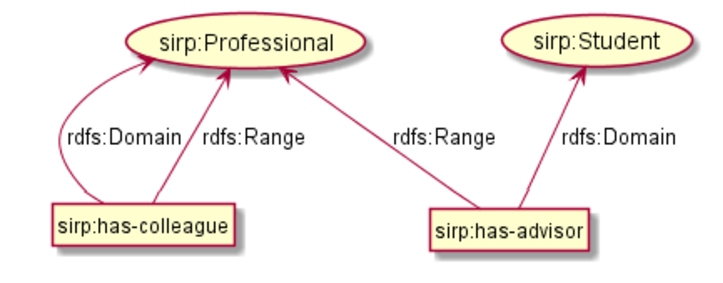
\includegraphics[scale=0.52]{exAxDyRPer}
	\end{figure}
	%%%%%%%%%%%%%%%%%%%%%%%
	
	\begin{figure}
	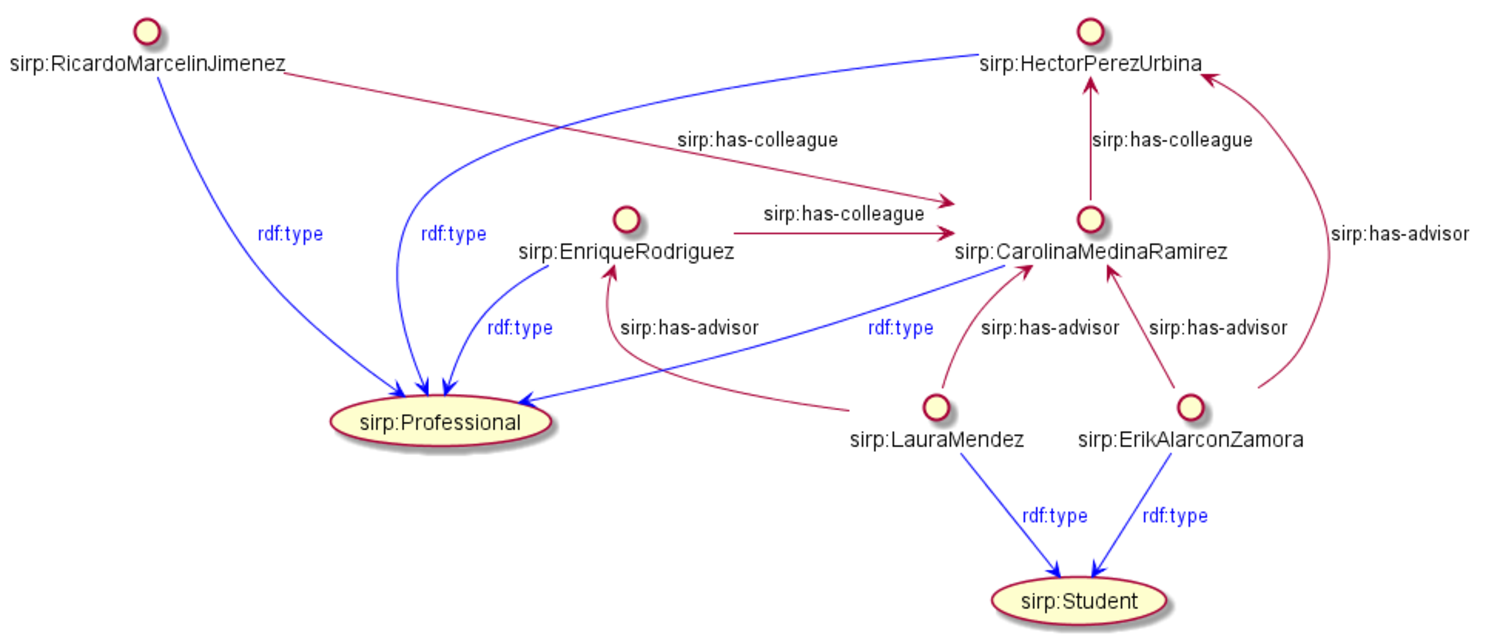
\includegraphics[scale=0.45]{exInfDyRPer}
	\end{figure}
	%%%%%%%%%%%%%%%%%%%%%%%
\end{frame}

\subsubsection{Caracter�sticas en las Propiedades}
\begin{frame}
	\frametitle{Caracter�sticas en las propiedades}
	\begin{block}{Propiedad sim�trica (owl:SymmetricProperty)}
	\justifying
	Afirma que la \textit{propiedad X} es su propia propiedad inversa, es decir, si la \textit{propiedad X} relaciona al \textit{individuo A} con el \textit{individuo B}, entonces, esta propiedad debe relacionar al \textit{individuo B} con el \textit{individuo A}.
	\end{block}
	
	\begin{figure}
	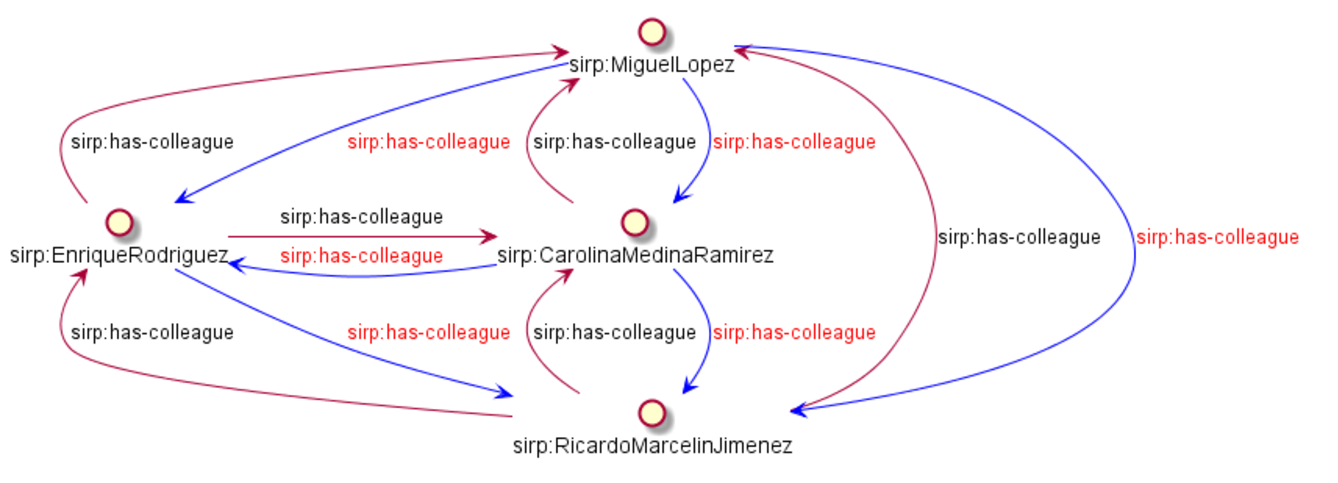
\includegraphics[scale=0.5]{infSymColl}
	\end{figure}
	%%%%%%%%%%%%%%%%%%%%%%%
\end{frame}
%%%%%%%%%%%%%%%%%%%%%%%%%%%%%%%%%%%%%%%%%%%%%%%%%%%%%%%%%%%%%%%%%%%%%%%%%%%%%%

\subsection{Buscar y recuperar la informaci�n en el modelo sem�ntico}
\begin{frame}
	\frametitle{Buscar y recuperar la informaci�n en el modelo sem�ntico}
%	\begin{block}{Objetivo}
%	\justifying
%	La b�squeda y recuperaci�n de la informaci�n para responder las preguntas o necesidades informativas de los usuarios del �rea de Redes y Telecomunicaciones (RyT).
%	\end{block}
	
	\begin{block}{SPARQL}
	\justifying 
	Lenguaje de consulta y protocolo de acceso a RDF, para la b�squeda y recuperaci�n de la informaci�n en un grafo RDF.
	\end{block}
	
	\begin{figure}
	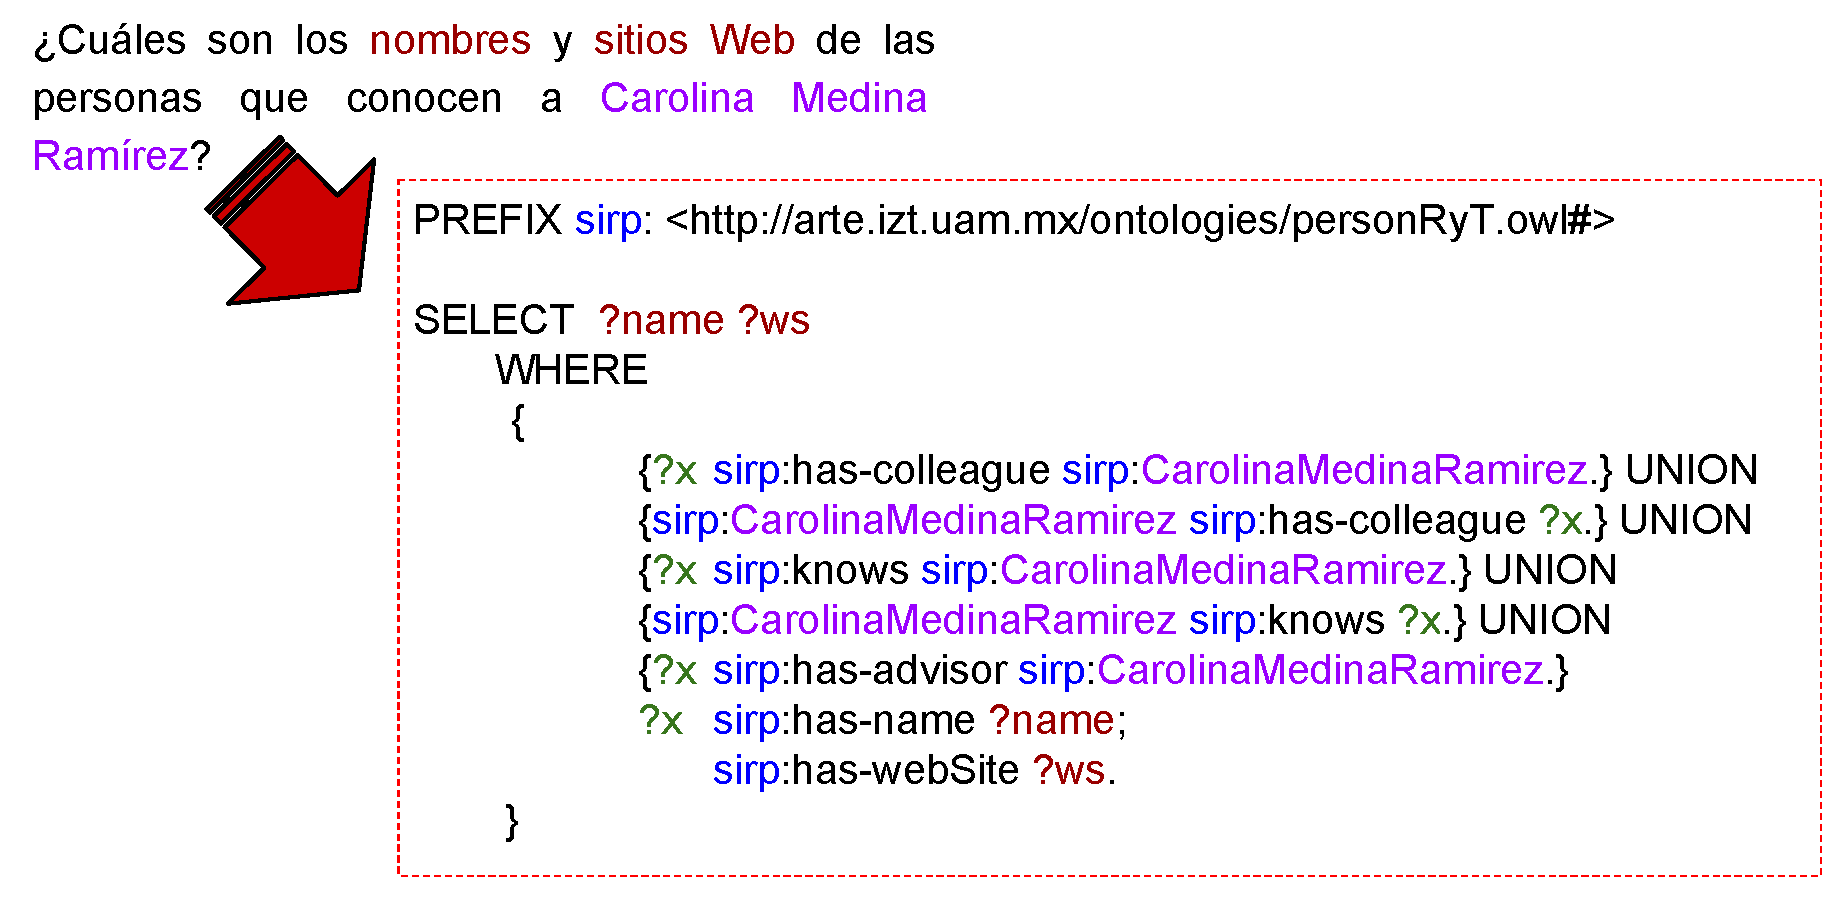
\includegraphics[scale=0.32]{q2rqlSR}
	\end{figure}
	
%	\begin{block}{Actividades}
%	\begin{enumerate}
%	\item \justifying Identificar las preguntas en lenguaje natural.
%	\item \justifying Transformar las preguntas a una consultas SPARQL.
%	\item \justifying Ejecutar las consultas mediante un motor de b�squeda SPARQL.
%	\end{enumerate}
%	\end{block}

\end{frame}

%%%%%%%%%%%%%%%%%%%%%%%%%%%%%%%%%%%%%%%%%%%%%%%%%%%%%%%%%%%%%%%%%%%%%%%%%%%%%%
\subsubsection{B�squeda + Inferencia}
\begin{frame}[allowframebreaks]
	\frametitle{Uso de inferencia}
		
	\begin{figure}
	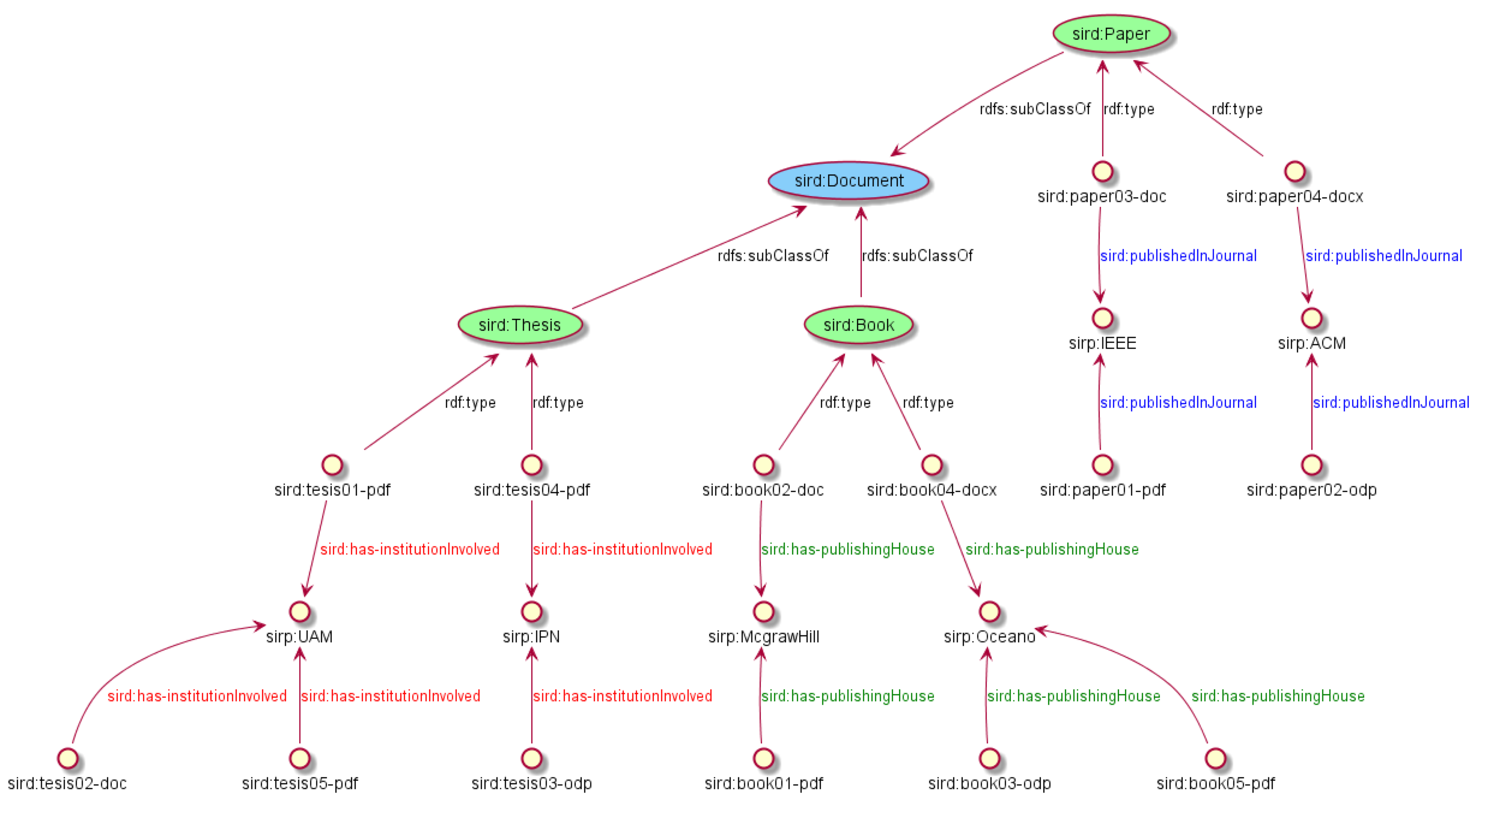
\includegraphics[scale=0.3]{grafoSR}
	\caption{Grafo RDF sin inferencia}
	\end{figure}
	%%%%%%%%%%%%%%%%%%%%%%%%%%%%%%%%%%%
	
	\begin{figure}[htbp]
	\centering
	\subfigure[Consulta sin inferencia]{
	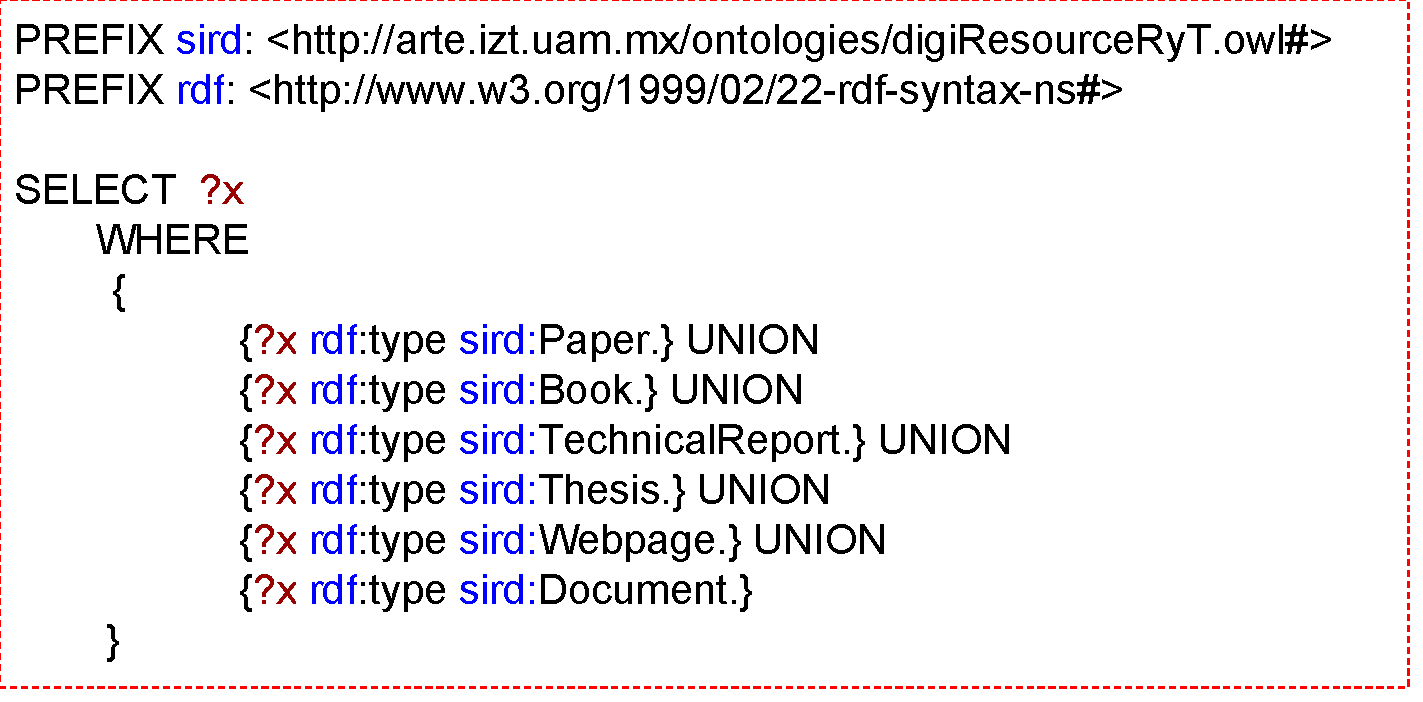
\includegraphics[scale=0.25]{consultaGrafo} 
	}
	\subfigure[Resultados de la consulta]{
	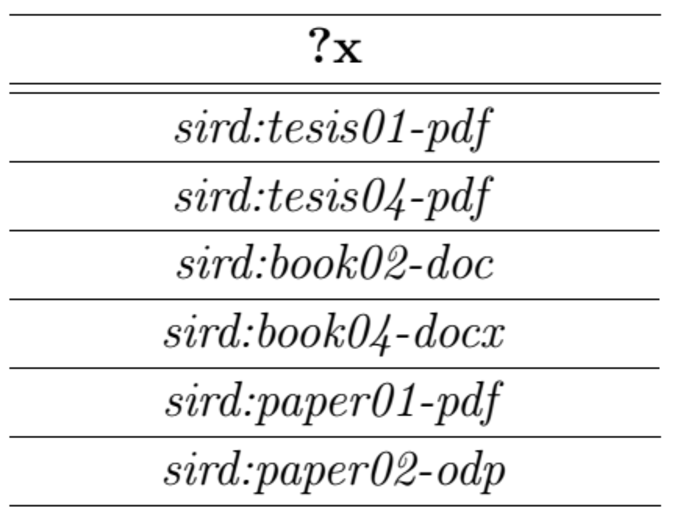
\includegraphics[scale=0.28]{RespQrySI} 
	}
	\end{figure}
	%%%%%%%%%%%%%%%%%%%%%%%%%%%%%%%%%%%
	
	\begin{figure}
	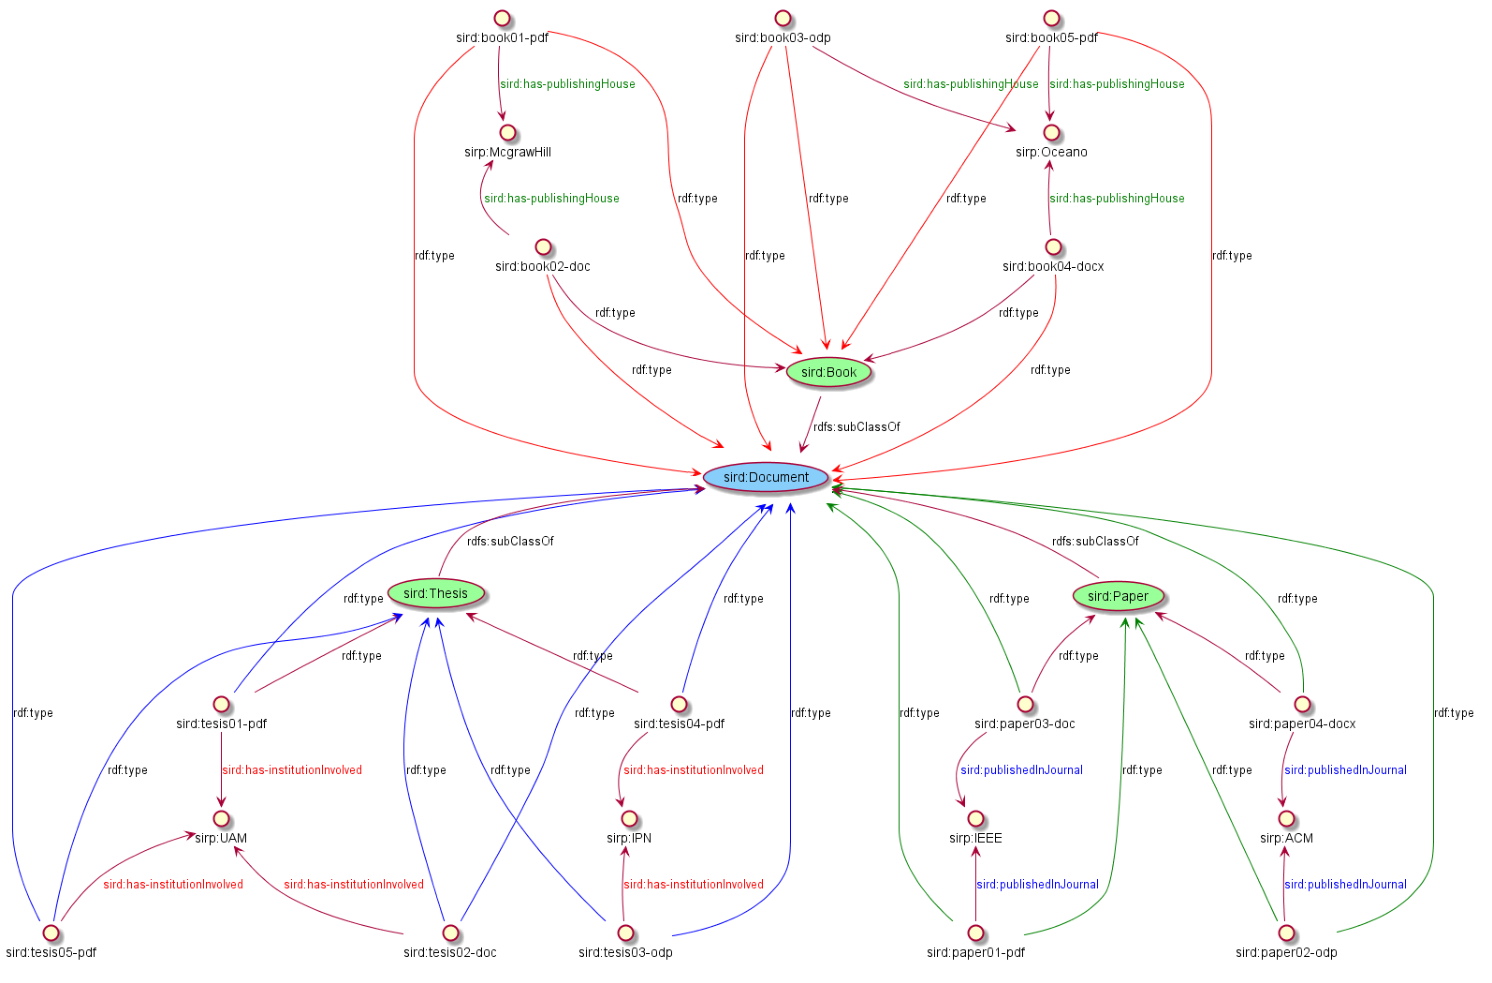
\includegraphics[scale=0.37]{grafoCR}
	\caption{Grafo RDF con inferencia}
	\end{figure}	
	%%%%%%%%%%%%%%%%%%%%%%%%%%%%%%%%%%%
\end{frame}

\subsubsection{Uso de inferencia IV}
\begin{frame}
	\frametitle{Uso de inferencia IV}
	\begin{figure}[htbp]
	\centering
	\subfigure[Consulta con inferencia]{
	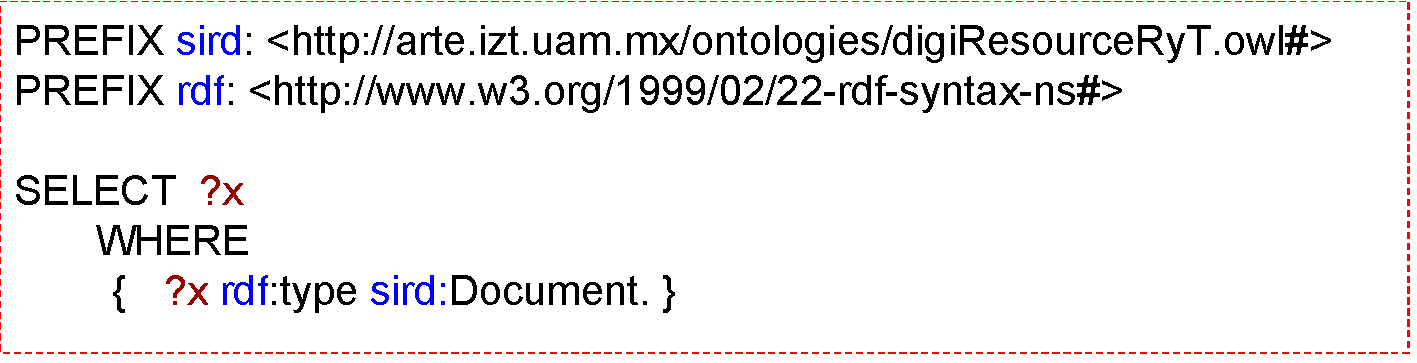
\includegraphics[scale=0.25]{consSimpGrafo} 
	}
	\subfigure[Resultados de la consulta]{
	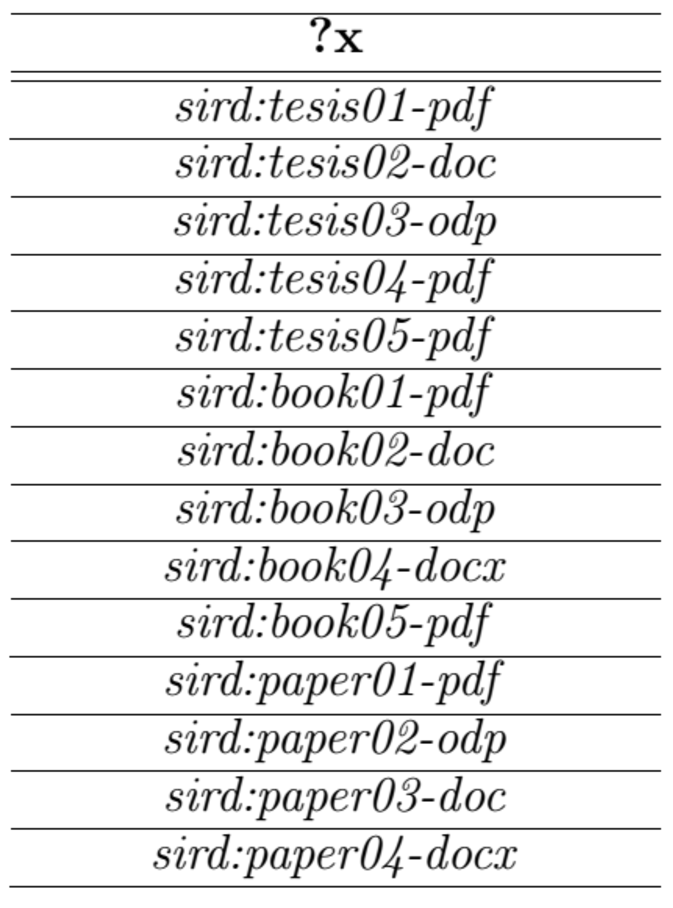
\includegraphics[scale=0.28]{RespQryCI} 
	}
	\end{figure}
\end{frame}
\chapter{Evaluaci�n experimental}
\label{cap:exp}
%%%% Observaci�n consiste en la medida y registro de hechos observables.
La \textit{integraci�n sem�ntica de los recursos} es el proceso de b�squeda y recuperaci�n de informaci�n en un \textit{grafo de conocimiento (ontolog�a)}. Un \textit{motor de b�squeda de tripletas} es el mecanismo encargado de realizar la consulta de informaci�n en los grafos de conocimiento, para responder una consulta dada. Este \textit{motor de tripletas} generalmente pertenece a un triplestore. En esta tesis, se emplea el \textit{triplestore Jena}; las razones de la elecci�n de Jena son presentadas en la Secci�n \ref{sec:eoats}. Jena proporciona dos componentes importantes: 1) \textit{un motor de b�squeda} para tripletas RDF y 2) \textit{un motor de inferencia} que soporta los axiomas en nuestras ontolog�as, los cuales son descritos en la Secci�n \ref{sec:enrKrec}.

\section{Observaciones}
El \textit{n�mero de los resultados} depende del uso o no de inferencia en nuestros modelos sem�nticos. Si Jena no hace uso de \textit{inferencia}, como el ejemplo de la Figura \ref{fig:grafoSR}, entonces el \textit{motor de b�squeda} puede proporcionar todos, varios o ning�n resultado. Esta variedad en la entrega de resultados, depende de las consultas SPARQL: 1) \textit{consultas sobre las declaraciones de los recursos}, como la consulta de la Figura \ref{fig:q112rql}, 2) \textit{consultas que agrupan varios patrones para un criterio de b�squeda}, como las consultas de las Figuras \ref{fig:q2rqlSR} y \ref{fig:q2torqlSR}, y 3) \textit{consultas simplificadas}, como en las Figuras \ref{fig:q2rqlCR} y \ref{fig:q2torqlCR}. En contraste, si Jena emplea inferencia, entonces puede entregar mejores resultados completos con respecto a la ontolog�a. Un ejemplo de este modelo se presenta en la Figura \ref{fig:grafoCR}.

Una caracter�stica asociada al uso de inferencia, es el impacto en el \textit{tiempo de procesamiento} de \textit{Jena} para responder las consultas. Por un lado, se ha observado que el \textit{tiempo de consulta} de Jena es peque�o, menor a medio segundo, cuando usa un \textit{modelo sin inferencia}. Mientras, el \textit{tiempo de consulta} de Jena para un \textit{modelo con inferencia} es mayor en comparaci�n con el tiempo del \textit{modelo sin inferencia}.

%%%% Hip�tesis es una soluci�n para un problema dado.
\section{Hip�tesis}
Con base en estas observaciones, nuestras dos hip�tesis de experimentaci�n  son �stas:
\begin{enumerate}
\item La \textit{inferencia} es un proceso importarte para la consulta de informaci�n mediante un triplestore que soporte a �sta.
%\textit{El \textbf{triplestore Jena} obtiene \textbf{resultados completos con respecto a la ontolog�a} cuando utiliza nuestros modelos con inferencia}.
\item El proceso de inferencia implica mayores tiempo de consulta, pero �stos son aceptables con Jena.
%\textit{El \textbf{tiempo de consulta} de Jena es \textbf{mayor} para nuestros \textit{modelos con inferencia} en comparaci�n con nuestros \textbf{modelos sin inferencia}}.
\end{enumerate}

%%%% M�todo consiste en: la elecci�n de los sujetos para confirmar la muestra, el procedimiento a seguir para �stos, las variables consideradas: dependiente, independiente y auxiliares.

%%Elaborar un experimento que ponga a prueba una hip�tesis
\section{Experimentaci�n}
Esta experimentaci�n consiste en la realizaci�n de dos actividades para probar nuestras hip�tesis de experimentaci�n. \textit{La \textbf{primera actividad} es \textbf{evaluar la calidad de los resultados} de Jena para los modelos con y sin inferencia}. Esta evaluaci�n consiste en estas etapas: 1) establecer una serie de consultas para interrogar nuestros modelos, 2) encontrar manualmente cu�ntos y cu�les recursos responden las consultas, 3) ejecutar las consultas con el motor ARQ de Jena y 4) comparar los recursos dados por Jena con las respuestas manuales.

\textit{La \textbf{segunda actividad} consiste en medir los \textbf{tiempos promedio de procesamiento} de Jena para las consultas de nuestra primera actividad}. La finalidad de esta segunda actividad es comparar los \textit{tiempos de consulta} para un modelo con inferencia y otro que no emplea �sta. En ambos modelos se eval�a el tiempo desde \textit{la ejecuci�n de Jena para una consulta a un modelo (con o sin inferencia)} hasta \textit{la presentaci�n de los resultados en pantalla}.

%%La determinaci�n del tiempo para modelos sin inferencia, consiste en medir los tiempos de: 1) \textit{ejecuci�n de la consulta en en el modelo} y 2) \textit{recuperaci�n de la informaci�n}. De la misma manera, la medici�n de tiempos para un modelo con inferencia es parecida a la medici�n en un modelos sin inferencia. La excepci�n es que en un modelo con inferencia, se toman en cuenta los tiempos para: \textit{el proceso de inferencia en el modelo} y \textit{la ejecuci�n de la consulta al modelo inferido}.

En esta tesis, el proceso de \textit{integraci�n sem�ntica} est� asociado a dos \textit{casos de uso} (cartograf�a de competencias y b�squeda de recursos digitales). Ahora bien, nuestra experimentaci�n consiste en probar la \textit{calidad de los resultados} y el \textit{tiempo de procesamiento} para la \textit{integraci�n sem�ntica de recursos} en la \textit{memoria corporativa} del �rea de Redes y Telecomunicaciones. Por esta raz�n, las dos actividades de nuestra experimentaci�n deben ser aplicadas a nuestros dos \textit{casos de uso}.

%%Elecci�n de los sujetos para confirmar la muestra
\section{Sujetos de experimentaci�n}
\label{sec:subexp} 
Los sujetos de nuestra experimentaci�n son un conjunto de ontolog�as que consisten en personas, documentos y archivos multimedia que son generados artificialmente. Esta \textit{generaci�n artificial} consiste en el uso de scripts para: 1) \textit{asignar un identificador URI para un conjunto de \textbf{recursos de informaci�n ficticios}} y 2) \textit{generar tripletas RDF para estos recursos con base en las \textbf{propiedades} y \textbf{clases} de nuestras ontolog�as, as� como \textbf{datos aleatorios}}. 

Un script genera un conjunto de declaraciones para los recursos persona. Mientras, otro script genera las declaraciones para los documentos y archivo multimedia. El algoritmo \ref{alg:fsg} presenta el funcionamiento general de ambos scripts para la generaci�n y almacenamiento de tripletas RDF.

\begin{algorithm}
\SetKwData{Sigma}{$\sigma_i$}
\SetKwData{Model}{$modelo_{rdf}$}
$N\leftarrow$  n�mero de \textit{recursos ficticios de informaci�n} a describir\;
\Model$\leftarrow$Crear un modelo rdf\;
\For{$i\leftarrow 1$ \KwTo $N$}{
	\Sigma$\leftarrow$Crear el recurso $i$ y establecer un identificador URI para �ste\;
	Elaborar los valores para cada caracter�stica significativa de este recurso (\Sigma)\; \label{lin:values}
	Escribir las aserciones, concatenando el URI del recurso (\Sigma), las propiedades de la ontolog�a y los valores del paso \ref{lin:values}\;
}
Guardar el \Model en un archivo con extensi�n ``\textit{rdf}'' y sintaxis de serializaci�n \textit{Turtle}\;
\caption{Funcionamiento b�sico de scripts para la generaci�n de tripletas artificialmente.}
\label{alg:fsg} 
\end{algorithm}

El ap�ndice \ref{aped:AlgDS} presenta los dos algoritmos con el funcionamiento detallado de los scripts. Un algoritmo para los datos simulados de los recursos persona y el otro para los recursos digitales.

La finalidad del uso de \textit{informaci�n simulada} es tener r�pidamente un volumen grande de datos en nuestros ABoxes. La \textit{cantidad de informaci�n} en estos ABox debe ser realista con respecto al �rea de Redes y Telecomunicaciones (RyT). Ya que al tener informaci�n realista, nuestra experimentaci�n se ajusta a la cantidad de datos que esperamos manejar en la integraci�n sem�ntica. Otra raz�n del uso de informaci�n simulada es ver si Jena soporta esta escala realista de datos. Esta \textit{escala de datos} se obtiene a partir de la media de \textit{recursos digitales} que un profesor del �rea de RyT utiliza en un trimestre, as� como el n�mero promedio de profesores y alumnos que hay en esta �rea.

Las cantidades de \textit{recursos persona} son 60 recursos artificiales y 13 recursos reales, dando un total de 73 personas. Mientras, las cantidades para los \textit{recursos digitales} son 16 recursos reales y 1314 recurso simulados, un total de 1330 recursos digitales.

En nuestra experimentaci�n, algunos \textit{recursos persona} tienen la declaraci�n que los asignan expl�citamente a una de estas clases: \textit{Estudiante (sirp:Student)}, \textit{Empleado (sird:Employee)} y \textit{Profesor (sirp:Teacher)}. Otros recursos persona carecen de esta asignaci�n, pero con inferencia �stos pueden clasificarse en una o varias clases de la \textit{ontolog�a cartograf�a de competencias}. De esta manera, se ve el impacto de hacer razonamiento.

En concreto, se tienen estas \textit{cantidades de recursos} por clase: 51 recursos son profesionistas y 23 son \textit{estudiantes}. Los 51 recursos persona mediante inferencia son asignados a la clase \textit{Profesionista (sirp:Professional)}. De estos 51 profesionistas se tiene que 19 son profesores y 9 son empleados. Por otro lado, de los 23 estudiantes se tiene que 9 recursos est�n asignados a la clase \textit{Estudiante} y los 14 restantes por inferencia son asignados a la clase \textit{Estudiante}. Existen 13 recursos persona que mediante inferencia se clasifican en la clase \textit{Investigador (sirp:Researcher)}.

La Tabla \ref{tab:noRP} muestra las cantidades de \textit{recursos persona} por clases de la \textit{ontolog�a cartograf�a de competencias}. La \textit{primera columna} presenta el nombre de las clases, la \textit{segunda} el n�mero de recursos que tienen la declaraci�n que los asigna expl�citamente a una clase y la \textit{tercera columna} el n�mero de recursos que por inferencia tienen la declaraci�n para asignarlos a una clase.

\begin{table}[!htb]
\renewcommand{\arraystretch}{1.2}
\centering
\begin{tabular}{| >{\centering\arraybackslash}m{2in} | >{\centering\arraybackslash}m{1.5in} | >{\centering\arraybackslash}m{1.5in} | }
\hline 
\multirow{2}{*}{\textbf{Clase}} & \multicolumn{2}{c|}{\textbf{N�mero de Recursos}} \\
\cline{2-3} 
 & \textbf{Sin inferencia} & \textbf{Con inferencia}\\
\hline 
\hline
Persona & 0 & 73\\
\hline
Investigador & 0 & 13\\
\hline
Profesionista & 0 & 51\\
\hline
Estudiante & 11 & 23\\
\hline
Profesor & 19 & 19\\
\hline
Empleado & 9 & 9\\
\hline
\end{tabular}
\caption{N�mero de recursos persona por clase.}
\label{tab:noRP}
\end{table}

De la misma manera que los \textit{recursos persona}, algunos \textit{recursos digitales} tienen la declaraci�n que los asignan expl�citamente a una clase. Otros recursos carecen de esta asignaci�n, pero con inferencia �stos pueden clasificarse en una o varias clases de la \textit{ontolog�a b�squeda de recursos digitales}.

Los 1330 recursos digitales de nuestra experimentaci�n se clasifican en: 156 art�culos, 366 libros, 34 reportes t�cnicos, 146 p�ginas web, 73 tesis, 42 videos, 42 audios, 77 im�genes y 112 presentaciones. De los 156 art�culos, 89 recursos tienen la declaraci�n expl�cita a la clase \textit{Art�culo (sird:Paper)} y los restantes 67 mediante inferencia tienen la declaraci�n a esta clase. En los libros, 185 recursos tienen la declaraci�n expl�cita y 181 recursos mediante inferencia tienen la declaraci�n a la clase \textit{Libro (sird:Book)}. De la misma manera, 79 recursos tienen la declaraci�n expl�cita a la clase \textit{P�gina Web (sird:PageWeb)} y 31 recursos a la clase \textit{Tesis (sird:Thesis)}. Mientras, 67 recursos mediante inferencia pertenecen a la clase  \textit{P�gina Web} y 42 a la clase \textit{Tesis}. Por �ltimo, los 1330 recursos se clasifican en 815 \textit{Documentos (sird:Document)} y 515 \textit{Multimedia (sird:Multimedia)}. Las declaraciones a estas dos clases se obtienen mediante inferencia.

La Tabla \ref{tab:noRD} presenta las cantidades de recursos digitales por clases de la \textit{ontolog�a recursos digitales}. Esta Tabla \ref{tab:noRD} presenta la misma estructura de la Tabla \ref{tab:noRP}.

\begin{table}[!htb]
\renewcommand{\arraystretch}{1.1}
\centering
\begin{tabular}{| >{\centering\arraybackslash}m{2in} | >{\centering\arraybackslash}m{1.5in} | >{\centering\arraybackslash}m{1.5in} | }
\hline 
\multirow{2}{*}{\textbf{Clase}} & \multicolumn{2}{c|}{\textbf{N�mero de Recursos}} \\
\cline{2-3} 
 & \textbf{Sin inferencia} & \textbf{Con inferencia}\\
\hline 
\hline
Recurso Digital & 0 & 1330\\
\hline
Documento & 0 & 815\\
\hline
Art�culo & 89 & 156\\
\hline
Reporte T�cnico & 34 & 34\\
\hline
P�gina Web & 79 & 146\\
\hline
Tesis & 31 & 73\\
\hline
Libro & 185 & 366\\
\hline
Multimedia & 0 & 515\\
\hline
Presentaci�n & 112 & 112\\
\hline
Audio & 42 & 42\\
\hline
V�deo & 42 & 42\\
\hline
Imagen & 77 & 77\\
\hline
\end{tabular}
\caption{N�mero de recursos digitales por clase.}
\label{tab:noRD}
\end{table}

\section{Metodolog�a}
Esta experimentaci�n se ha dividido en dos actividades. La primera actividad consiste en la \textit{evaluaci�n de la calidad de los resultados} que proporciona el triplestore Jena. Mientras, la segunda actividad consiste en medir los \textit{tiempos promedios} que toma Jena para: consultar los modelos con/sin inferencia y mostrar los resultados al usuario.

El \textit{primer paso} en la \textit{evaluaci�n de la calidad de resultados} es identificar un conjunto b�sico de consultas para interrogar las ontolog�as \textit{cartograf�a de competencias} y \textit{b�squeda de recursos digitales}. En la Secci�n \ref{sec:byrKrec} se hizo un an�lisis e identificaci�n de preguntas base que posteriormente se transformaron a consultas SPARQL. Estas consultas de la Secci�n \ref{sec:byrKrec} son reutilizadas para la primer actividad de esta experimentaci�n.

El \textit{segundo paso} es encontrar cu�ntos y cu�les recursos son relevantes para responder las consultas de nuestra experimentaci�n. Para ello, se hace una \textit{b�squeda manual} exhaustiva de los recursos relevantes que responden las consultas de experimentaci�n. Esta b�squeda se hace sobre los recursos de nuestra memoria corporativa que est� guiada por los casos de uso. Para cada consulta, se anotan los identificadores URI de los \textit{recursos relevantes} y la cantidad de �stos.

La Tabla \ref{tab:qrynoRP} muestra las preguntas base para la \textit{cartograf�a de competencias}. En esta Tabla, la primera columna presenta el identificador para cada una de las diecinueve preguntas, la segunda columna enuncia la pregunta y la tercer columna presenta el n�mero de recursos que responden a �sta. De la misma manera, la Tabla \ref{tab:qrynoRD} presenta un identificador, las preguntas y cantidad de recursos que responden a �stas, para la \textit{b�squeda de recursos digitales}. En estas dos Tablas, no se presentan los identificadores URI de los recursos que responden a las preguntas, porque algunas consultas tienen muchos recursos relevantes.

\begin{table}[!hp]
\renewcommand{\arraystretch}{1.4}
\centering
\begin{tabular}{>{\centering\arraybackslash}m{1in} >{\arraybackslash}m{3.5in} >{\centering\arraybackslash}m{1in}}
\hline 
Id. Consulta & Pregunta & No. de Recursos\\
\hline
\hline 
Q1.1 &  �Cu�les el nombre, correo, sitio web, g�nero y edad de las personas del �rea de RyT? & 73 \\
\hline
Q1.2 & �Cu�l es el nombre, sitio web y el lugar donde laboran las personas del RyT? & 73\\
\hline 
Q1.3 & �Qui�nes son mayores de 20 a�os y menores de 45 a�os? & 50\\
\hline 
Q1.4 & �Qui�nes son profesionistas del �rea de RyT? & 51\\
\hline 
Q1.5 & �Qui�nes trabajan en Clark \& Parsia y son del sexo Masculino? & 3\\
\hline 
Q1.6 & �Qui�nes son estudiantes y leen en ingl�s? & 8\\
\hline 
Q1.7 & �Quienes hablan, leen y escriben en ingl�s? & 16\\
\hline 
Q1.8 & �Qu� estudiantes saben algo de ingl�s? & 6\\
\hline 
Q1.9 & �Qu� profesores tienen la capacidad de s�ntesis? & 2\\
\hline 
Q1.10 & �Qu� profesionistas tienen conocimiento en los temas de Web Sem�ntica? & 58\\
\hline
Q1.11 & �Qu� profesores tienen conocimientos en Sistemas Distribuidos? & 3\\
\hline 
Q1.12 & �Qui�nes tienen conocimiento en Java, OWL, RDF, Threads, C, OpenMP? & 1\\
\hline 
Q1.13 & �Qu� estudiantes tienen alg�n conocimiento en los subtemas de Sistemas Operativos? & 33\\
\hline 
Q1.14 & �Qui�nes trabajan en una Universidad? & 24\\
\hline 
Q1.15 & �Quienes laboran en la UAM y tienen alg�n conocimiento en  Web Sem�ntica? & 19\\
\hline 
Q1.16 & �Qu� personas tienen como asesor a Carolina Medina? & 2\\
\hline 
Q1.17 & �Qui�nes son los colegas de Ricardo Marcelin? & 8\\
\hline 
Q1.18 &  �Qui�nes conocen a Carolina Medina Ramirez? & 11\\
\hline 
Q1.19 & �Qu� personas son profesores-investigadores? & 9\\
\hline 
\end{tabular}
\caption{Preguntas y cantidad de personas que responden a �stas.}
\label{tab:qrynoRP}
\end{table}

\begin{table}[!hp]
\renewcommand{\arraystretch}{1.4}
\centering
\begin{tabular}{>{\centering\arraybackslash}m{1in} >{\arraybackslash}m{3.5in} >{\centering\arraybackslash}m{1in}}
\hline 
Id. Consulta & Pregunta & No. de Recursos\\
\hline
\hline 
Q2.1 & �Cu�les son los t�tulos, rutas, extensi�n, idioma de todos los recursos digitales de RyT? & 1330 \\
\hline
Q2.2 & �Cu�les libros tratan sobre algunos temas de Sistemas Distribuidos? & 103\\
\hline 
Q2.3 & �Qu� recursos fueron publicados por la UAM? & 18\\
\hline 
Q2.4 & �Qu� documentos son para dar un curso de Sistemas P2P? & 31\\
\hline 
Q2.5 & �Qu� recursos multimedia son mayores al a�o 2009? & 119\\
\hline 
Q2.6 & �Cu�les documentos tratan sobre Ontolog�as? & 30\\
\hline 
Q2.7 & �Qu� recursos fueron publicados en una Revista cient�fica? & 156\\
\hline 
Q2.8 & �Qu� recursos tienen en su contenido las palabras "linked data"? & 159\\
\hline 
Q2.9 & �Cu�les documentos en ingl�s y mayores al a�o 2000 son de autor�a de Erik Alarc�n Zamora? & 2\\
\hline 
Q2.10 & �Cu�les la tesis de Samuel Hern�ndez Maza? & 4\\
\hline 
\end{tabular}
\caption{Preguntas y cantidad de recursos digitales que responden a �stas.}
\label{tab:qrynoRD}
\end{table}

En el Anexo \ref{aped:TrPC}, se presentan las consultas SPARQL que est�n asociadas a cada pregunta de las Tablas \ref{tab:qrynoRP} y \ref{tab:qrynoRD}.

El \textit{tercer paso} es emplear \textit{Jena} para ejecutar las \textit{consultas SPARQL} a un modelo sin inferencia y otro con inferencia. La finalidad de esto es ver la calidad de resultados y la cantidad de �stos que al emplear un modelo con inferencia y otro sin inferencia. De esta manera, podemos ver el impacto de la inferencia para la consulta de informaci�n en una ontolog�a.

En esta \textit{ejecuci�n de consultas}, se emplea un script para consultar un \textit{modelo sem�ntico} y proporcionar los resultados que est�n asociados a una consulta dada. El funcionamiento de este script se presenta en el Algoritmo \ref{alg:srinf}. En este algoritmo, los \textbf{\textit{par�metros de entrada}} son: 1) \textit{la consulta SPARQL}, 2) \textit{la ontolog�a} (\textit{Personas o RecDigi}), 3) \textit{inferencia} (\textit{0 sin inferencia} y \textit{1 con inferencia}). Mientras, los par�metros de salida son: 1) \textit{los identificadores URI que responden la consulta} y 2) \textit{la cantidad de recursos respuesta}. Este script permite ejecutar una consulta a la vez por corrida e imprime los par�metros de salida en pantalla.

\begin{algorithm}
\SetKwData{Model}{$modelo_{semantico}$}
\KwIn{Consulta SPARQL: $query$, Nombre del modelo: $model$, Uso de inferencia: $inference$}
\KwOut{Resultados: $\Pi_{query}$, N�mero de resultados: $noRes$}
\BlankLine
$noRes \leftarrow 0, \Pi_{query} \leftarrow \{ \}$\;
\uIf{$model \equiv$ `Personas'}{
	Cargar en memoria el ABox y TBox de la ontolog�a cartograf�a de competencias\;
}
\ElseIf{$model \equiv$ `RecDigi'}{
	Cargar en memoria el ABox y TBox de la ontolog�a b�squeda de recursos digitales\;
}
\uIf{$inference \equiv 0$}{
	\Model $\leftarrow$ modelo ABox y TBox\;
}
\ElseIf{$inference \equiv 1$}{
	Inferir en memoria sobre el ABox y TBox\;
	\Model $\leftarrow$ modelo inferido\;
}
Cargar en memoria consulta SPARQL ($query$)\;
Ejecutar consulta ($query$) en el modelo (\Model)\;
$\Pi_{query} \leftarrow$ Recuperar resultados de consulta\tcc*{$\Pi_{query} = \{ \pi_1, \dots, \pi_n \}$}
\ForAll{elements of $\Pi_{query}$}{
	Imprimir $\pi_k$ en pantalla\;
	$noRes \leftarrow noRes + 1$\;
}
Imprimir $noRes$ en pantalla\;
\caption{Algoritmo para la evaluaci�n de la calidad de resultados}
\label{alg:srinf} 
\end{algorithm}

El \textit{cuarto paso} es comparar los \textit{resultados que proporciona el script (Algoritmo \ref{alg:srinf})} con los \textit{resultados que sabemos responden (b�squeda manual)} las consultas de las Tablas \ref{tab:qrynoRP} y \ref{tab:qrynoRD}. La finalidad de este paso, es \textit{evaluar} la calidad de resultados de Jena, para un modelo con inferencia y otro sin el uso de �sta. El cuarto paso, se hace en dos fases: 1) \textit{encontrar los recursos relevantes} de las respuestas dadas por el script, y 2) usar (\textit{m�tricas de recuperaci�n de la informaci�n}) para comparar la calidad de los resultados con y sin inferencia. 

La \textit{fase uno} consiste en comparar y anotar las cantidades de recursos relevantes para cada consulta. En esta fase se considera el modelo de uso: con inferencia o sin �sta. Esta comparaci�n y anotaci�n se hizo de forma manual. El primer criterio de comparaci�n es ver la cantidad de recursos de las Tablas \ref{tab:qrynoRP} y \ref{tab:qrynoRD} con el n�mero de respuestas que proporciona el script. Posteriormente, se hace la comparaci�n \textit{identificador} a \textit{identificador} de \textit{los recursos que son proporcionados por el script} con \textit{los recursos que se saben responden a la consulta}.

La segunda fase, consiste en emplear dos m�tricas de \textit{recuperaci�n de la informaci�n (RI\label{sym:ri})}:

\begin{itemize}
\item La \textbf{\textit{exhaustividad (recall)}} \cite{Nasraoui} es ``\textit{la cantidad de elementos relevantes que han sido recuperados, entre la cantidad de elementos relevantes en la base de conocimientos}'' \cite{RecYPres}. La exhaustividad se presenta en la Ecuaci�n \ref{ec:exa}.

\begin{equation}
	Exhaustividad = \frac{N\acute{u}mero\: de\: recursos\: relevantes\: que\: han\: sido\: recuperados}{N\acute{u}mero\: de\: recursos\: relevantes\: en\: la\: base\: de\: conocimientos} * 1.0
	\label{ec:exa}
\end{equation}

\end{itemize}

\begin{itemize}
\item La \textbf{\textit{precisi�n (precision)}} \cite{Nasraoui} es la ``\textit{cantidad de elementos recuperados que son relevantes, entre el total de elementos recuperados}'' \cite{RecYPres}. La precisi�n se presenta en la Ecuaci�n \ref{ec:pre}.

\begin{equation}
	Precisi�n = \frac{N\acute{u}mero\: de\: elementos\: relevantes\: que\: han\: sido\: recuperados}{Total\: de\:elementos\: recuperados\: en\: la\: base\: de\: conocimientos} *1.0
	\label{ec:pre}
\end{equation}
\end{itemize}

En las ecuaciones de la exhaustividad y precisi�n, los divisores y dividendos son elementos que se han encontrado en esta primer actividad. En concreto, �stos son los elementos en las dos ecuaciones:

\begin{itemize}
\item \textit{Exhaustividad}: La \textit{cantidad de elementos relevantes recuperados} es el \textit{n�mero de recursos relevantes que proporciona el script para una consulta}; esta informaci�n se obtiene en el etapa uno de este cuarto paso. Mientras, el n�mero de \textit{elementos relevantes en la base de conocimiento} es la \textit{cantidad de resultados de nuestra b�squeda manual} que est�n en las Tablas \ref{tab:qrynoRP} y \ref{tab:qrynoRD}.
\item \textit{Precisi�n}: La \textit{cantidad de elementos relevantes recuperados} es el \textit{n�mero de recursos relevantes que proporciona el script para una consulta}. Mientras, \textit{el total de elementos recuperados en la base de conocimiento} es la cantidad de \textit{recursos dados por el script, sin el an�lisis de los recursos relevantes}.
\end{itemize}

El objetivo de emplear estas dos m�tricas, es evaluar las capacidades de \textit{recuperaci�n de la informaci�n} del triplestores Jena. En particular, la \textit{exhaustividad} eval�a la habilidad de Jena para encontrar los recursos relevantes en una ontolog�a, mientras la \textit{precisi�n} eval�a la habilidad de Jena para filtrar los recursos relevantes \cite{Cleverdon68}.

En esta experimentaci�n, la \textbf{segunda actividad} es tomar los tiempos de procesamiento para la consulta y recuperaci�n de informaci�n en un modelo sem�ntico a partir del uso de Jena. El objetivo de esta actividad es comparar estos tiempos de consulta para un modelo con inferencia y otro sin el uso de �sta.

Los tiempos importantes en esta actividad son la medici�n desde \textit{la consulta de informaci�n en un modelo sem�ntico con Jena} hasta \textit{la impresi�n de los resultados en pantalla}. Esta medici�n de los tiempos, se hace con base en la modificaci�n del script del Algoritmo \ref{alg:srinf}. Porque este Algoritmo \ref{alg:srinf} lleva a cabo todo el proceso de b�squeda y recuperaci�n de la informaci�n relevante en los \textit{recursos de informaci�n}. Tambi�n, este Algoritmo permite elegir el modelo: si es cero, entonces no hay inferencia y si es uno, se emplea inferencia.

El funcionamiento del \textit{script modificado} es tomar `\textbf{\textit{n}}' veces el \textit{tiempo de procesamiento} cuando se consulta un modelo sem�ntico (con o sin inferencia). Posteriormente, este script calcula y regresa el \textit{tiempo promedio de consulta} para una \textit{consulta SPARQL} dada. El Algoritmo \ref{alg:mod} presenta el funcionamiento de este script modificado.

\begin{algorithm}
\SetKwData{Model}{$modelo_{semantico}$}
\SetKwFunction{time}{time}
\KwIn{Consulta SPARQL: $query$, Nombre del modelo: $model$, Uso de inferencia: $inference$, N�mero de repeticiones: $N$}
\KwOut{Tiempo promedio: $Tiempo_{promedio}$}
\BlankLine
$\Pi_{query} \leftarrow \{ \}$\;
$t_{ini} \leftarrow 0, t_{fin} \leftarrow 0, Tiempo_{promedio} \leftarrow 0$\;
\For{$i\leftarrow 1$ \KwTo $N$}{
	\uIf{$model \equiv$ `Personas'}{
		Cargar en memoria el ABox y TBox de la ontolog�a cartograf�a de competencias\;
	}
	\ElseIf{$model \equiv$ `RecDigi'}{
		Cargar en memoria el ABox y TBox de la ontolog�a b�squeda de recursos digitales\;
	}
	\uIf{$inference \equiv 0$}{
		\Model $\leftarrow$ modelo ABox y TBox\;
	}
	\ElseIf{$inference \equiv 1$}{
		Inferir en memoria sobre el ABox y Tbox\;
		\Model $\leftarrow$ modelo inferido\;
	}
	Cargar en memoria consulta SPARQL ($query$)\;
	
	$t_{ini} \leftarrow$ \time{}\;
	Ejecutar consulta ($query$) en el modelo (\Model)\;
	$\Pi_{query} \leftarrow$ Recuperar resultados de consulta\tcc*{$\Pi_{query} = \{ \pi_1, \dots, \pi_n \}$}
	\ForAll{elements of $\Pi_{query}$}{
		Imprimir $\pi_k$ en pantalla\;
	}
	$t_{fin} \leftarrow$ \time{}\;
	$Tiempo_{promedio} \leftarrow Tiempo_{promedio} + (t_{fin} - t_{ini})$\;
}
\Return $Tiempo_{promedio}$\;
\caption{Algoritmo para medir el tiempo promedio en el proceso de consulta.}
\label{alg:mod} 
\end{algorithm}

%consiste en medir los \textbf{tiempos promedio de procesamiento} de Jena para las consultas de nuestra primera actividad}. La finalidad de esta segunda actividad es comparar los \textit{tiempos de consulta} para un modelo con inferencia y otro que no emplea �sta. En ambos modelos se eval�a el tiempo desde \textit{la ejecuci�n de Jena para una consulta a un modelo } hasta \textit{la presentaci�n de los resultados en pantalla}.

Este script (Algoritmo \ref{alg:mod}) se ejecuta para cada una de las consultas que est�n asociadas a las preguntas en las Tablas \ref{tab:qrynoRP} y \ref{tab:qrynoRD}. Porque, este script permite procesar una consulta a la vez. El n�mero de repeticiones se establece en 20 ($N = 20$). Mientras, las modelos empleados son las ontolog�as de \textit{cartograf�a de competencias} y \textit{b�squeda de recursos digitales}. El par�metro importante es el uso o no de inferencia para el modelo sem�ntico.

Los scripts asociados a los Algoritmos \ref{alg:srinf} y \ref{alg:mod}, se corrieron en una computadora con un procesador Intel Core I7 a 2.3GHz con 8Gb en RAM y 8 n�cleos de procesamiento. La versi�n del Apache Jena es la 2.7.4 para Windows 7 (64bits). Estos scripts se construyeron con el IDE Eclipse y se ejecutaron con la versi�n 1.7.0\_05 de Java.

\section{Resultados}
Los resultados para la \textit{evaluaci�n de la calidad de los resultados} se presentan en dos etapas. Estas dos etapas tienen relaci�n con las dos fases del cuarto paso de esta evaluaci�n. La primera etapa presenta la cantidad de resultados (relevantes y el total) que fueron recuperados por el script del Algoritmo \ref{alg:srinf}. La segunda etapa presenta los valores calculados para la exhaustividad y precisi�n. Este c�lculo se hace para cada consulta de la experimentaci�n.

\begin{table}[!htb]
\renewcommand{\arraystretch}{0.92}
\centering
\begin{tabular}{| >{\centering\arraybackslash}m{1in} | >{\centering\arraybackslash}m{1in} | >{\centering\arraybackslash}m{1in} | >{\centering\arraybackslash}m{1in} | >{\centering\arraybackslash}m{1in} | }
\hline 
\multirow{2}{*}{\textbf{Id. Consulta}} & \multicolumn{2}{c|}{\textbf{Modelo sin inferencia}} & \multicolumn{2}{c|}{\textbf{Modelo con inferencia}}\\
\cline{2-5} 
 & \textbf{Recursos relevantes} & \textbf{Total recursos recuperados} & \textbf{Recursos relevantes} & \textbf{Total recursos recuperados}\\
\hline 
\hline
Q1.1 & 73 & 73 & 73 & 73\\
\hline
Q1.2 & 73 & 73 & 73 & 73\\
\hline
Q1.3 & 50 & 50 & 50 & 50\\
\hline
Q1.4 & 28 & 28 & 51 & 51\\
\hline
Q1.5 & 3 & 3 & 3 & 3\\
\hline
Q1.6 & 4 & 4 & 8 & 8\\
\hline
Q1.7 & 16 & 16 & 16 & 16\\
\hline
Q1.8 & 2 & 2 & 6 & 6\\
\hline
Q1.9 & 10 & 10 & 10 & 10\\
\hline
Q1.10 & 2 & 2 & 58 & 58\\
\hline
Q1.11 & 3 & 3 & 3 & 3\\
\hline
Q1.12 & 1 & 1 & 1 & 1\\
\hline
Q1.13 & 6 & 6 & 20 & 20\\
\hline
Q1.14 & 16 & 16 & 24 & 24\\
\hline
Q1.15 & 2 & 2 & 2 & 2\\
\hline
Q1.16 & 2 & 2 & 2 & 2\\
\hline
Q1.17 & 2 & 2 & 8 & 8\\
\hline
Q1.18 & 7 & 7 & 11 & 11\\
\hline
Q1.19 & 0 & 0 & 13 & 13\\
\hline
\end{tabular}
\caption{Recursos relevantes y no relevantes asociados a las preguntas de la cartograf�a de competencias.}
\label{tab:rrRP}
\end{table}

En la Tabla \ref{tab:rrRP} se presentan las cantidades de recursos relevantes y totales de la primera etapa, para las preguntas de la Tabla \ref{tab:qrynoRP}. La primer columna presenta el identificador de consulta. La segunda y tercera columna muestra la cantidad de recursos relevantes y total recursos recuperados cuando se emplea un modelo sin inferencia. La cuarta y quinta presentan los recursos relevantes y total de recursos recuperados para un modelo con inferencia.

De la misma manera, la Tabla \ref{tab:rrRD} presenta la cantidad de recursos relevantes y total de recursos recuperados cuando se consulta el modelo sin inferencia y con inferencia de los recursos digitales. En esta Tabla, las consultas est�n asociadas a las preguntas de la Tabla \ref{tab:qrynoRD}. La estructura de la Tabla \ref{tab:rrRD} es igual a la Tabla \ref{tab:rrRP}.

\begin{table}[!htb]
\renewcommand{\arraystretch}{0.94}
\centering
\begin{tabular}{| >{\centering\arraybackslash}m{1in} | >{\centering\arraybackslash}m{1in} | >{\centering\arraybackslash}m{1in} | >{\centering\arraybackslash}m{1in} | >{\centering\arraybackslash}m{1in} | }
\hline 
\multirow{2}{*}{\textbf{Id. Consulta}} & \multicolumn{2}{c|}{\textbf{Modelo sin inferencia}} & \multicolumn{2}{c|}{\textbf{Modelo con inferencia}}\\
\cline{2-5} 
 & \textbf{Recursos relevantes} & \textbf{Total recursos recuperados} & \textbf{Recursos relevantes} & \textbf{Total recursos recuperados}\\
\hline 
\hline
Q2.1 & 1330 & 1330 & 1330 & 1330\\
\hline
Q2.2 & 0 & 0 & 103 & 103\\
\hline
Q2.3 & 18 & 18 & 18 & 18\\
\hline
Q2.4 & 15 & 15 & 31 & 31\\
\hline
Q2.5 & 66 & 66 & 119 & 119\\
\hline
Q2.6 & 15 & 15 & 30 & 30\\
\hline
Q2.7 & 156 & 156 & 156 & 156\\
\hline
Q2.8 & 159 & 159 & 159 & 159\\
\hline
Q2.9 & 0 & 0 & 2 & 2\\
\hline
Q2.10 & 3 & 3 & 4 & 4\\
\hline
\end{tabular}
\caption{Recursos relevantes y no relevantes asociados a las preguntas de la b�squeda de recursos digitales.}
\label{tab:rrRD}
\end{table}

Los resultados para la segunda etapa de la \textit{evaluaci�n de la calidad de resultados}, son los valores que fueron calculados para la exhaustividad (Ecuaci�n \ref{ec:exa}) y precisi�n (Ecuaciones \ref{ec:pre}) de Jena con nuestras ontolog�as. El objetivo de esta \textit{segunda etapa} es comparar estas dos m�tricas de \textit{recuperaci�n de la informaci�n} para un modelo con inferencia y otro que no usa �sta, donde estos modelos son procesados por Jena.

La Tabla \ref{tab:exprRP} muestra los valores de exhaustividad y precisi�n para las consultas en la Tabla \ref{tab:qrynoRP}. En esta Tabla \ref{tab:exprRP}, la primer columna muestra el identificador de la consulta. La segunda y tercera columna muestran los valores de exhaustividad y precisi�n para un modelo sin inferencia. La cuarta y quinta columna presentan los valores de las mismas m�tricas para un modelo con inferencia.

\begin{table}[!htb]
\renewcommand{\arraystretch}{0.92}
\centering
\begin{tabular}{| >{\centering\arraybackslash}m{1in} | >{\centering\arraybackslash}m{1.2in} | >{\centering\arraybackslash}m{1in} | >{\centering\arraybackslash}m{1.2in} | >{\centering\arraybackslash}m{1in} | }
\hline 
\multirow{2}{*}{\textbf{Id. Consulta}} & \multicolumn{2}{c|}{\textbf{Modelo sin inferencia}} & \multicolumn{2}{c|}{\textbf{Modelo con inferencia}}\\
\cline{2-5} 
 & \textbf{Exhaustividad} & \textbf{Precisi�n} & \textbf{Exhaustividad} & \textbf{Precisi�n}\\
\hline 
\hline
Q1.1 & 1 & 1 & 1 & 1\\
\hline 
Q1.2 & 1 & 1 & 1 & 1\\
\hline 
Q1.3 & 1 & 1 & 1 & 1\\
\hline 
Q1.4 & 0.549 & 1 & 1 & 1\\
\hline 
Q1.5 & 1 & 1 & 1 & 1\\
\hline 
Q1.6 & 0.5 & 1 & 1 & 1\\
\hline 
Q1.7 & 1 & 1 & 1 & 1\\
\hline 
Q1.8 & 0.333 & 1 & 1 & 1\\
\hline 
Q1.9 & 1 & 1 & 1 & 1\\
\hline 
Q1.10 & 0.034 & 1 & 1 & 1\\
\hline 
Q1.11 & 1 & 1 & 1 & 1\\
\hline 
Q1.12 & 1 & 1 & 1 & 1\\
\hline 
Q1.13 & 0.3 & 1 & 1 & 1\\
\hline 
Q1.14 & 0.666 & 1 & 1 & 1\\
\hline 
Q1.15 & 1 & 1 & 1 & 1\\
\hline 
Q1.16 & 1 & 1 & 1 & 1\\
\hline 
Q1.17 & 0.25 & 1 & 1 & 1\\
\hline 
Q1.18 & 0.636 & 1 & 1 & 1\\
\hline 
Q1.19 & 0 & - & 1 & 1\\
\hline
\end{tabular}
\caption{Exhaustividad y precisi�n para las consultas de la cartograf�a de competencias.}
\label{tab:exprRP}
\end{table}

De la misma manera, la Tabla \ref{tab:exprRD} presenta los valores de estas dos m�tricas de RI, para las preguntas de la Tabla \ref{tab:qrynoRD}. Estos valores est�n asociados al modelo de \textit{b�squeda de recursos digitales}. La estructura de esta Tabla \ref{tab:exprRD} es la misma de la Tabla \ref{tab:exprRP}.

\begin{table}[!htb]
\renewcommand{\arraystretch}{0.92}
\centering
\begin{tabular}{| >{\centering\arraybackslash}m{1in} | >{\centering\arraybackslash}m{1.2in} | >{\centering\arraybackslash}m{1in} | >{\centering\arraybackslash}m{1.2in} | >{\centering\arraybackslash}m{1in} | }
\hline 
\multirow{2}{*}{\textbf{Id. Consulta}} & \multicolumn{2}{c|}{\textbf{Modelo sin inferencia}} & \multicolumn{2}{c|}{\textbf{Modelo con inferencia}}\\
\cline{2-5} 
 & \textbf{Exhaustividad} & \textbf{Precisi�n} & \textbf{Exhaustividad} & \textbf{Precisi�n}\\
\hline 
\hline
Q2.1 & 1 & 1 & 1 & 1\\
\hline 
Q2.2 & 0 & - & 1 & 1\\
\hline 
Q2.3 & 1 & 1 & 1 & 1\\
\hline 
Q2.4 & 0.484 & 1 & 1 & 1\\
\hline 
Q2.5 & 0.555 & 1 & 1 & 1\\
\hline 
Q2.6 & 0.5 & 1 & 1 & 1\\
\hline 
Q2.7 & 1 & 1 & 1 & 1\\
\hline 
Q2.8 & 1 & 1 & 1 & 1\\
\hline 
Q2.9 & 0 & - & 1 & 1\\
\hline 
Q2.10 & 0.75 & 1 & 1 & 1\\
\hline
\end{tabular}
\caption{Exhaustividad y precisi�n para las consultas de la b�squeda de recursos digitales.}
\label{tab:exprRD}
\end{table}

Las Tablas \ref{tab:tiempRP} y \ref{tab:tiempRD} presentan los resultados de \textit{evaluar los tiempos promedio de procesamiento}. La Tabla Tablas \ref{tab:tiempRP} muestra los tiempos promedio de consulta para las preguntas en la Tabla \ref{tab:qrynoRP}. De la misma manera, la Tabla \ref{tab:tiempRD} muestra los tiempos para las preguntas en la Tabla \ref{tab:qrynoRD}. El objetivo de esta evaluaci�n es comparar los tiempos al consultar un modelo sin inferencia y otro con inferencia.

La estructura es la misma para las Tablas \ref{tab:tiempRP} y \ref{tab:tiempRD}. �sta es la estructura de estas Tablas: la primer columna muestra el identificador de la consulta, la segunda el tiempo promedio al consultar un modelo sin inferencia y la tercer columna el tiempo promedio de consulta en un modelo obtenido por inferencia.

\begin{table}[!htb]
\renewcommand{\arraystretch}{0.92}
\centering
\begin{tabular}{| >{\centering\arraybackslash}m{2in} | >{\centering\arraybackslash}m{2in} | >{\centering\arraybackslash}m{2in} | }
\hline 
\multirow{2}{*}{\textbf{Id. Consulta}} & \multicolumn{2}{c|}{\textbf{Tiempo promedio (milisegundos)}} \\
\cline{2-3} 
 & \textbf{Modelo sin inferencia} & \textbf{Modelo con inferencia}\\
\hline 
\hline
Q1.1 & 13 & 133\\
\hline
Q1.2 & 17 & 152\\
\hline
Q1.3 & 12 & 138\\
\hline
Q1.4 & 10 & 194\\
\hline
Q1.5 & 7 & 140\\
\hline
Q1.6 & 7 & 125\\
\hline
Q1.7 & 8 & 125\\
\hline
Q1.8 & 9 & 126\\
\hline
Q1.9 & 6 & 123\\
\hline
Q1.10 & 6 & 136\\
\hline
Q1.11 & 7 & 124\\
\hline
Q1.12 & 6 & 125\\
\hline
Q1.13 & 8 & 406\\
\hline
Q1.14 & 8 & 128\\
\hline
Q1.15 & 6 & 126\\
\hline
Q1.16 & 9 & 127\\
\hline
Q1.17 & 25 & 125\\
\hline
Q1.18 & 28 & 129\\
\hline
Q1.19 & 7 & 157\\
\hline
\end{tabular}
\caption{Tiempo promedio de procesamiento para las consultas de la cartograf�a de competencias.}
\label{tab:tiempRP}
\end{table}

\begin{table}[!htb]
\renewcommand{\arraystretch}{0.92}
\centering
\begin{tabular}{| >{\centering\arraybackslash}m{2in} | >{\centering\arraybackslash}m{2in} | >{\centering\arraybackslash}m{2in} | }
\hline 
\multirow{2}{*}{\textbf{Id. Consulta}} & \multicolumn{2}{c|}{\textbf{Tiempo promedio (milisegundos)}} \\
\cline{2-3} 
 & \textbf{Modelo sin inferencia} & \textbf{Modelo con inferencia}\\
\hline 
\hline
Q2.1 & 24 & 3520\\
\hline
Q2.2 & 9 & 4016\\
\hline
Q2.3 & 12 & 3520\\
\hline
Q2.4 & 16 & 3472\\
\hline
Q2.5 & 42 & 3451\\
\hline
Q2.6 & 14 & 3392\\
\hline
Q2.7 & 13 & 3431\\
\hline
Q2.8 & 32 & 3312\\
\hline
Q2.9 & 34 & 3570\\
\hline
Q2.10 & 11 & 3398\\
\hline
\end{tabular}
\caption{Tiempo promedio de procesamiento para las consultas de la b�squeda de recursos digitales.}
\label{tab:tiempRD}
\end{table}

El an�lisis de las Tablas \ref{tab:rrRP}, \ref{tab:rrRD}, \ref{tab:tiempRP} y \ref{tab:tiempRD} arroja varios aspectos significativo con relaci�n a los \textit{recursos relevantes recuperados}. En el caso del uso de modelos sin inferencia se tiene los siguientes hechos. 1) En algunos casos, una consulta al conocimiento expl�cito recupera todos los recursos relevantes y los tiempos de respuesta son peque�os (no pasan del segundo). 2) En otros casos, algunas consultas descartan varios recursos que s� responden la consulta. Esto se debe a que algunos recursos carecen un determinado tripleta.

En el caso de uso de inferencia, Jena permite recuperar todos los recursos esperados, porque el motor de inferencia permite inferir algunos triples en \textit{nuestras ontolog�as}. Estos triples inferidos son criterios de b�squeda las consultas de nuestra experimentaci�n. Pero, el uso de inferencia consume mayor tiempo, porque el \textit{motor de b�squeda} invierte mayor tiempo en inferir m�s tripletas de nuestros grafos RDF.

%%%%%---------------------> Aqu� hay que responder
%�Cu�l es la conclusi�n? �Vale la pena pagar el precio del razonamiento? �Cu�ndo ser� mejor hacer el razonamiento? �Al momento de ejecutar la consulta? �No ser� mejor tal vez materializar todo desde el principio y olvidarnos?


%Todo tiene un costo, cuando el razonador materializa los triples en el modelo, �ste consume tiempo en procesamiento y al hacer una consulta, el motor debe comparar m�s aserciones. El desarrollador no debe abusar de la axiomatizaci�n, en algunos casos cuando la consulta es sobre  hechos expl�citos, no es necesario el uso del razonador, basta con escribir y hacer la consulta sobre el conocimiento expl�cito.

%La primer conclusi�n afirma que el performance mejora cuando se usan axiomas. Esta afirmaci�n resulta cierta, porque un razonador deduce una relaci�n que vincula directamente dos objetos. An�logamente, resulta m�s r�pido ir por el camino directo que por una serie de rutas hasta el mismo objeto.

%La segunda conclusi�n tiene que ver con el n�mero de resultados. Si bien, las aserciones establecen un conjunto directo y est�tico de enlaces entre los distintos recursos de nuestro modelo. En muchas ocasiones, al momento de construir una consulta SPARQL no se contemplan algunos de estos enlaces, inclusive en otros casos, estos enlaces no est�n escritos expl�citamente. Por consiguiente, mucho recursos no se contemplan como respuesta para una consulta. En contraste, los axiomas, aserciones y un razonador, establecen estos enlaces entre recursos de forma expl�cita en memoria, de esta manera, las consultas respondan m�s resultados que no se


\chapter{Conclusiones y Recomendaciones}
\label{cap:concl}
Con base en lo realizado y descrito en este documento, nosotros concluimos lo siguiente:

\begin{itemize}
\item Los objetivos particulares se alcanzaron:
	\begin{itemize}
	\item Desarrollamos un \textit{marco de referencia} para la \textit{integraci�n sem�ntica} de los \textit{recursos de informaci�n} existentes en una \textit{memoria corporativa}.
	\item Implementamos un \textit{modelo sem�ntico} que representa el conocimiento expl�cito e impl�cito de los \textit{recursos de informaci�n}.
	\item Implementamos un prototipo de interfaz gr�fica de usuario que permite a los usuarios una interacci�n amigable para la integraci�n sem�ntica de los recursos de informaci�n.
	\item Evaluamos los resultados devueltos y tiempos de procesamiento en la integraci�n sem�ntica para el dominio de redes y telecomunicaciones.
	\end{itemize}
\item Con respecto a nuestro objetivo principal, decimos que al alcanzar nuestros objetivos particulares, nosotros contribuimos a la \textit{integraci�n sem�ntica} de los \textit{recursos de informaci�n} existentes en una memoria corporativa.
\item La hip�tesis \textbf{El uso de las \textit{tecnolog�as sem�nticas} es adecuado para lograr la \textit{integraci�n sem�ntica} de \textit{recursos de informaci�n} en una \textit{memoria corporativa}}, se acepta porque las tecnolog�as sem�nticas son herramientas, est�ndares, metodolog�as y aplicaciones que permiten:
	\begin{itemize}
	\item Representar el conocimiento expl�cito (caracter�sticas y/o relaciones) de los \textit{recursos de informaci�n} en un modelo sem�ntico; solucionando las dificultades de heterogeneidad en formato, contenido y estructura.
	\item Enriquecer el conocimiento, mediante la introducci�n de \textit{reglas de inferencia} (Ver Secci�n \ref{sec:reginf} y \ref{sec:enrKrec}) en el modelo sem�ntico, para representar el conocimiento impl�cito en los recursos y el dominio de aplicaci�n (Redes y Telecomunicaciones).
	\item Extender o modificar un modelo sem�ntico, gracias a que el conocimiento expl�cito e impl�cito est�n escritos en un lenguaje est�ndar (Ver Secciones \ref{sec:rdf} y \ref{sec:reginf}). De esta manera, los modelos sem�nticos pueden adaptarse al conocimiento cambiante o explosivo de la memoria corporativa.
	\item Compartir un modelo sem�ntico, gracias a que �ste est� escrito en un lenguaje est�ndar y puede utilizarse en cualquier plataforma (Linux, Mac y Windows). De esta manera, mediante el uso de aplicaciones gen�ricas se puede visualizar o modificar la informaci�n en el modelo.
	\item Buscar y recuperar informaci�n en un modelo sem�ntico, mediante el uso de un lenguaje est�ndar (Ver Secci�n \ref{sec:lsparql}). As� como, el uso de un proceso para hacer expl�cito el conocimiento impl�cito de un modelo sem�ntico, con la finalidad de mejorar los resultados de la b�squeda en el modelo (Ver Secci�n \ref{sec:result}).
	\end{itemize}
\item Las aportaciones de nuestra investigaci�n son:
	\begin{itemize}
	\item Un \textit{marco de referencia} para lograr la integraci�n sem�ntica de recursos de informaci�n.
	\item Un modelo sem�ntico (ontolog�a) que representa el conocimiento de una memoria corporativa (Redes y Telecomunicaciones).
	\item Un prototipo para la b�squeda y consulta de informaci�n.
	\item Los resultados de nuestra evaluaci�n experimental.
	\item Un par de scripts para la generaci�n autom�tica y controlada de descripciones RDF, para poblar la base de conocimiento.
	\end{itemize}
\end{itemize}

%%%Qu� hicimos
En este documento presentamos un estudio y aplicaci�n sobre el uso de las \textit{tecnolog�as sem�nticas} (TS) para realizar la \textit{integraci�n sem�ntica} de los \textit{recursos de informaci�n} en una \textit{memoria corporativa}. Por \textit{integraci�n sem�ntica} debe entenderse la \textit{b�squeda y recuperaci�n} significativa de informaci�n existente en los \textit{recursos de informaci�n}. Estos recursos son documentos basados en texto y archivos multimedia en diferentes formatos, con contenido variado y con distintas estructuras (estructurado, semi-estructurado, sin estructura), tambi�n otros recursos de informaci�n en este trabajo son las personas.

%%%Por qu� hicimos �sto
Este trabajo tiene dos finalidades. Por un lado, esta investigaci�n propone un modelo sem�ntico (ontolog�a) que representa el conocimiento de una memoria corporativa, correspondiente al dominio de aplicaci�n de Redes y Telecomunicaciones. Conocimiento residente en personas y recursos digitales. Por otro lado, hacer la \textit{b�squeda y recuperaci�n inteligente de informaci�n} para responder las preguntas de los usuarios de la memoria.

%%Nuestro prototipo realmente f�cilita la interacci�n entre usuarios y un modelo sem�ntico.
As� mismo, nuestro trabajo propone un \textit{marco de referencia} para lograr la \textit{integraci�n sem�ntica de recursos} en una \textit{memoria corporativa}. Esta propuesta comprende tres actividades. La primera actividad es construir un modelo para representar el \textit{conocimiento expl�cito} de los \textit{recursos de informaci�n} existentes en una memoria corporativa. La segunda actividad es introducir \textit{reglas de inferencia} para enriquecer al modelo con conocimiento impl�cito existente en la memoria corporativa. La tercera actividad es \textit{buscar y recuperar informaci�n} existente en la memoria corporativa mediante la interrogaci�n del modelo sem�ntico.

%%%Qu� hicimos en cada etapa con las tecnolog�as sem�nticas
%%%Ventajas del uso de las tecnolog�as sem�nticas

Nosotros decidimos explorar las \textit{tecnolog�as sem�nticas} para la integraci�n de \textit{recursos de informaci�n} dadas las ventajas siguientes:

\begin{itemize}
\item El \textit{est�ndar RDF} permite representar cualquier recurso, sea un ser vivo, un archivo digital, un pa�s, ciudad, un edificio, una organizaci�n o un concepto abstracto. De esta manera, se contribuye a la integraci�n de informaci�n de \textit{recursos de informaci�n} que son heterog�neos en formato, contenido y estructura.
\item El \textit{est�ndar RDF} establece que los recursos tengan un identificador �nico de recurso (URI), para identificar de manera �nica a un recurso. De esta forma, se solucionan problemas de homonimia con respecto a los nombres de los recursos.
\item La representaci�n del contenido (caracter�sticas) de los \textit{recursos de informaci�n} de una memoria corporativa no se limita a un peque�o n�mero de caracter�sticas sobre �stos; sino que pueden vincularse estos recursos con otros a trav�s de relaciones o caracter�sticas m�s espec�ficas.
\item La introducci�n de \textit{reglas de inferencia} en la ontolog�a para enriquecer el conocimiento representado a trav�s de ella, ya que un razonador a partir de estas reglas puede hacer expl�cito el conocimiento impl�cito.
\item Una \textit{ontolog�a} puede ser extendida con el fin de \textit{incorporar mayor conocimiento} o \textit{adaptarse a cambios en el conocimiento}. De esta manera, si nuevos recursos se describen, entonces �stos pueden incorporarse a la ontolog�a. Ahora bien, si cambia el conocimiento en algunas ramas de la ontolog�a, entonces �stas pueden ser sustituidas por otras.
\item Una \textit{ontolog�a} est� escrita en un lenguaje est�ndar (OWL o RDF(S)) y representan un vocabulario consensuado por los expertos. Por esta raz�n, �stas se pueden intercambiar y reutilizar entre personas y/o aplicaciones.
\item Una \textit{ontolog�a} puede representarse de varias formas: a trav�s de un grafo dirigido o \textit{tripletas} (sujeto predicado objeto), cualquiera de ellas permite comprender los recursos as� como las reglas de inferencia.
\item Una \textit{ontolog�a} fomenta el desarrollo de aplicaciones gen�ricas para aprovechar estos modelos. Ejemplos de estas aplicaciones son editores de ontolog�as, interfaces gr�ficas para describir sem�nticamente los recursos, navegadores sobre ontolog�as, por mencionar algunas. Estas herramientas gen�ricas posibilitan que personas expertas en el dominio sean las principales constructoras del grafo de conocimiento. De esta manera, la informaci�n en el grafo ser� confiable, ya que estas personas son las que tienen los conocimientos en el dominio.
\end{itemize}

%Otras ventajas de tener ontolog�as en un formato est�ndar, son:
%\begin{itemize}
%\item Realizar tareas de inferencia a partir de los vocabularios OWL y RDF(S).
%\item Liberar a las organizaciones del uso de formatos propietarios que tienen un costo econ�mico o de propiedad intelectual.
%\item Construir r�pidamente modelos de conocimiento a partir de ontolog�as b�sicas.
%\item Mezclar ontolog�as y construir modelos de conocimiento complejos.
%\end{itemize}

%%%Ventajas de nuestra propuesta en relaci�n a otros trabajos
%Este \textit{marco de trabajo} emplea a los \textit{casos de uso} para guiar el proceso de \textit{integraci�n sem�ntica}. El primer \textit{caso de uso} es la \textit{cartograf�a de competencias} que consiste en encontrar personas con base a sus habilidades y capacidades profesionales, as� como conocimientos en los temas del dominio de la memoria. El segundo caso es la \textit{b�squeda de recursos digitales} que consiste en encontrar los \textit{documentos y recursos multimedia} a partir de la informaci�n sobre �stos (metadatos), en particular, encontrar recursos por los temas del dominio en la memoria.

%Estos dos \textit{casos de uso} son independientes entre s�, por ello, este marco propone la construcci�n de dos modelos u ontolog�as. La primera ontolog�a tiene el conocimiento expl�cito e impl�cito acerca de los \textit{recursos persona}. De la misma manera, la segunda ontolog�a tiene el conocimiento de los \textit{recursos digitales}. Un aspecto importante en ambos \textit{casos de uso} es vincular a cualquier recurso con los temas del dominio de la memoria corporativa. Por esta raz�n, se construye una tercera ontolog�a con los temas del dominio, donde estos temas est� jerarquizados.

%%%Para qui�n lo hicimos y con que prop�stio
%Esta propuesta se implemento para la memoria corporativa del �rea de Redes y Telecomunicaciones que pertenece al departamento de Ingenier�a El�ctrica de la Universidad Aut�noma Metropolitana. Por ello, la primera ontolog�a tiene informaci�n sobre profesores, alumnos y colegas que est�n vinculados con esta �rea. La segunda ontolog�a tienen informaci�n sobre los recursos digitales que representan trabajos, investigaciones, notas de curso, proyectos, tesis de las personas del �rea RyT. La tercera ontolog�a tiene los temas del �rea de RyT que est�n jerarquizados en cuatro ramas: \textit{sistemas distribuidos}, redes y servicios de telecomunicaciones, sistemas de comunicaci�n digital y web sem�ntica.

%%% que ventajas tiene nuestro prototipo en relacion con otros que se han examinado
La tarea de b�squeda y recuperaci�n de informaci�n son actividades que no cualquier usuario puede llevar a cabo, porque es necesario que tenga conocimientos sobre las tecnolog�as sem�nticas, as� como estar familiarizado en el dominio de conocimiento. Por esta raz�n, nosotros proponemos en esta investigaci�n un modelo (ontolog�a de Redes y Telecomunicaciones) y un prototipo (aplicaci�n) para permitir la interacci�n de cualquier usuario con el modelo, con fines de b�squeda y recuperaci�n de informaci�n en la memoria corporativa de trabajo (Redes y Telecomunicaciones).

La interfaz de nuestro prototipo est� orientada al usuario, es decir, un ambiente visual que permite una manera agradable para consultar la informaci�n de los recursos en nuestra ontolog�a. Esta caracter�stica es importante, porque en los trabajos de nuestro \textit{estado del arte} (Ver Secci�n \ref{sec:eoaisr}), ninguna aplicaci�n est� orientada al usuario.

Este prototipo establece las siguientes funcionalidades: 1) permitir a los usuarios, navegar a trav�s de la informaci�n b�sica en los \textit{recursos de informaci�n}, 2) permitir a los usuarios, estructurar sus preguntas y hacer b�squedas espec�ficas de los recursos, 3) publicar los resultados de la b�squeda y navegaci�n en un formato visual agradable, 4) transformar la preguntas a consultas SPARQL, 5) cargar las ontolog�as en memoria, 6) emplear un razonador para hacer expl�cito el conocimiento impl�cito de nuestro modelo sem�ntico.

%%%Conclusiones sobre la experimentaci�n
Nosotros llevamos a cabo una evaluaci�n experimental. Los objetivos de esta evaluaci�n son: 1) \textit{evaluar la calidad de los resultados de Jena para los modelos con y sin inferencia}, as� como 2) \textit{medir los tiempos promedio de procesamiento de Jena para las consultas de nuestra primera actividad}. En la medici�n de tiempos, quer�amos ver el rendimiento de Jena con la cantidad de datos que esperamos manejar. Mientras, en la evaluaci�n de resultados, quer�amos ver si los resultados devueltos por Jena, son los que responden nuestras preguntas.

Los resultados en nuestra experimentaci�n indican lo siguiente. El \textit{tiempo de consulta} es mayor en un \textit{modelo con inferencia} en comparaci�n con un \textit{modelo sin inferencia}. Sin embargo, los resultados de las b�squedas en un modelo sin inferencia son variados. En algunos casos, todos los \textit{resultados} que se sabe responden la consulta, son recuperados cuando la consulta es sobre el conocimiento expl�cito. En otros casos, recursos que responden la consulta, son descartados dado que estos recursos carecen de su descripci�n (tripleta) en la base de conocimiento. En cambio, los resultados de b�squedas sobre un \textit{modelo con inferencia} son buenos, porque estas consultas recuperan todos los recursos que de antemano sabemos que responden a las consultas; a pesar de no tener una descripci�n (tripleta) en la base de conocimiento.

Respecto a los tiempos, se tiene lo siguiente: el proceso de consulta sin inferencia arroja tiempos menores a un segundo, mientras los tiempos en la consulta con inferencia son de al rededor de dos o tres segundos. Aunque, los tiempos con inferencia son mayores en comparaci�n de los tiempos sin inferencia, a�n estos tiempos con inferencia son aceptables para la b�squeda de informaci�n basada en ontolog�as.

%%%Conclusi�n final, es factible o no es factible el uso de las TS y describir porqu�

%En este trabajo presentamos nuestro \textit{marco de trabajo}, un prototipo para la consulta de informaci�n, los resultados en nuestra evaluaci�n experimental, as� como las ventajas de las tecnolog�as sem�nticas, y con base en �stos, nosotros hacemos esta conclusi�n. 

%%% Trabajos futuros
\section{Recomendaciones}
En esta investigaci�n, nosotros identificamos varias actividades que consideramos como trabajos futuros:

\begin{itemize}
\item \textbf{A corto plazo:}
	\begin{itemize}
	\item Introducir m�s \textit{casos de uso}, por ejemplo, la administraci�n del inventario en los distintos laboratorios que componen el departamento de ingenier�a el�ctrica de la UAM.
	\item Actualizar los \textit{recursos de informaci�n} y las descripciones de �stos, para tener una buena representaci�n de la memoria corporativa del �rea de Redes y Telecomunicaciones.
	\item Evaluar la introducci�n de \textit{reglas de inferencia} m�s complejas en la ontolog�a, mediante el an�lisis de las reglas existentes y el uso de reglas del lenguaje \textit{Semantic Web Rule Language} \cite{SWRL} (SWRL), por ejemplo, si X es pariente de Z y Y tiene como hermano a K, entonces X es sobrino de K.
	\item Mejorar el prototipo de integraci�n sem�ntica de recursos:
		\begin{itemize}
		\item Agregar un cuadro para hacer b�squedas por palabras clave, mediante Lucene Index \cite{Lucene}.
		\item Optimizar los \textit{tiempos de procesamiento} en la b�squeda, por ejemplo, generando nuevas tripletas (materializando) desde el inicio las tripletas y almacen�ndolas en un nuevo modelo.
		\item Mejorar la manera en que se muestra la informaci�n de los recursos respuesta para una pregunta dada, mediante el uso del plug-in DataTables \cite{DataTables}.
		\item Mejorar la seguridad en la interfaz Web: autenticaci�n, autorizaci�n y administraci�n de sesiones, mediante el uso del marco de seguridad Apache Shiro \cite{Shiro}.
	\end{itemize}
	\end{itemize}
\item \textbf{A mediano plazo:}
	\begin{itemize}
	\item Automatizar la caracterizaci�n de los \textit{recursos de informaci�n}, mediante el uso de miner�a de texto.
	\item Mejorar la interfaz gr�fica de usuario del prototipo para que �ste pueda describir los \textit{recursos de informaci�n}. El objetivo es que los usuarios empleen esta aplicaci�n como una del estilo ``red social''. Algunas funcionalidades de esta interfaz son:
		\begin{itemize}
			\item Describir un nuevo \textit{recurso de informaci�n}.
			\begin{itemize}
				\item Asignar un identificador �nico de recurso al nuevo recurso de informaci�n.
				\item Construir un conjunto de tripletas RDF, asociadas al nuevo recurso de informaci�n.
				\item Guardar las tripletas en un archivo o agregar inmediatamente �stas al modelo sem�ntico.
			\end{itemize}
			\item Actualizar la informaci�n de un \textit{recurso de informaci�n}.
			\begin{itemize}
				\item Corregir la informaci�n en el modelo.
				\item Guardar el nuevo modelo.
			\end{itemize}
			\item Eliminar las descripciones de un \textit{recurso de informaci�n}.
			\begin{itemize}
				\item Ver la informaci�n del recurso a eliminar.
				\item Eliminar las tripletas en el modelo, donde el recurso es el sujeto.
				\item Guardar el nuevo modelo.
			\end{itemize}
		\end{itemize}
	\item Utilizar otro triplestore, por ejemplo Stardog \cite{Clark} o Sesame \cite{Aduna}, y hacer una evaluaci�n del mismo.
		\begin{itemize}
		\item Cargar, inferir y consultar nuestras ontolog�as con el \textit{triplestore electo}.
		\item Hacer nuestra evaluaci�n experimental con este triplestore.
		\item Comparar el desempe�o y resultados de experimentaci�n del \textit{triplestore electo} contra \textit{Jena}.
		\end{itemize}
	\item Dar mantenimiento a la ontolog�a del vocabulario de Redes y Telecomunicaciones.
		\begin{itemize}
		\item Introducir nuevos conceptos, como radios cognitivos, computaci�n en la nube, computaci�n m�vil, por mencionar algunos.
		\item Introducir tripletas para traducir los conceptos de nuestra ontolog�a a otros idiomas, por ejemplo, semantic web, web sem�ntica, web sem\^{a}ntica, semantisch web, anlamsal web, web semantikoa. De esta manera, en una b�squeda se pueden enriquecer los resultados, recuperando recursos que est�n en otros idiomas.
		\end{itemize}
	\end{itemize}
\end{itemize}

%%%%%%%%%%----------->Hay que expandir el cap�tulo con m�s ventajas de las TS

%Este cap�tulo est� bien escrito en general; pero es demasiado concreto. Hay que expandir las ventajas de la utilizaci�n de las tecnolog�as sem�nticas para vender la tesis mejor :).

%\section{Referencias}
%\begin{frame}[allowframebreaks]
%\frametitle{Referencias}
%\begin{scriptsize} \bibliographystyle{apalike}
%\justifying \bibliography{bibliografia}\end{scriptsize}
%\end{frame}

\end{document}
